\documentclass[]{dukedissertation}
%\documentclass[economy,twoside,bind]{dukedissertation}
% Use the second for a single-spaced copy suitable for duplex printing
% and binding.

% Other useful options (there are more options documented in Chapter 2):
%  * draft -- don't actually include images, print a black bar on overfull
%             hboxes
%  * MS    -- Format for a Master's Thesis.  No UMI abstract page, some 
%             textual changes to title page.  


% Useful packages for dissertation writing:
\usepackage{amsmath, amssymb, amsfonts, amsthm}
\usepackage{graphicx}
\usepackage{natbib}
\usepackage{color}
\usepackage{bm}
\usepackage{subfigure}
\usepackage{graphicx}
\usepackage{mathabx}
\usepackage{multirow}
\usepackage{setspace}
\usepackage{tabularx}
\usepackage{wrapfig}
\usepackage{dblfloatfix}
\usepackage{booktabs}
\usepackage{adjustbox}
\usepackage{lscape} 
\usepackage{rotating}

%---------------- show page layout. don't use in a real document!
%\usepackage{showframe}
%\renewcommand\ShowFrameLinethickness{0.15pt}
%\renewcommand*\ShowFrameColor{\color{red}}
%---------------------------------------------------------------%
    
% \usepackage{cite}  % If you include this, hyperlink cites will
                     % break.  It's nice to use this package if your bibstyle
							% sorts entries by order-of-use, rather than
							% alphabetically (as plain does).
							
%Theorem, Lemma, etc. environments
\newtheorem{theorem}{Theorem}%[section]
\newtheorem{lemma}[theorem]{Lemma}
\newtheorem{proposition}[theorem]{Proposition}
\newtheorem{corollary}[theorem]{Corollary}
\newtheorem{result}[theorem]{Result}

% Personal commands and abbreviations.
%Define and personal commands here

%Graphics Path to find your pictures
\graphicspath{{./Pictures/}}

%Italics sans serif to get rid of nasty curls in default italic numerals
\usepackage{xparse}
\ExplSyntaxOn
\NewDocumentCommand \italicize { m }
  { \nathdwek_italicize:n { #1 } }
\cs_new_protected:Npn \nathdwek_italicize:n #1
 {
  \tl_set:Nn \l_tmpa_tl { #1 }
  \tl_map_inline:nn { 0123456789 }
   { \tl_replace_all:Nnn \l_tmpa_tl { ##1 } { \textsl { ##1 } } }
  \textit { \tl_use:N \l_tmpa_tl }
 }
\ExplSyntaxOff

\newcommand\blfootnote[1]{%
  \begingroup
  \renewcommand\thefootnote{}\footnote{#1}%
  \addtocounter{footnote}{-1}%
  \endgroup
}

\hyphenpenalty=9500

%-----------------------------------------------------------------------------%
% PREAMBLE 
%-----------------------------------------------------------------------------%
\author{Daniel Aaron Snellings}
\title{Somatic Mutations Drive Vascular Malformation \\Initiation, Progression, and Predisposition}
\supervisor{Douglas Marchuk}
\department{Molecular Genetics and Microbiology} % Appears as Department of \department
% Declare dissertation subject used on UMI abstract page.  List of
% categories: http://dissertations.umi.com/duke/subject_categories.html
%\subject{[Your Subject Here]}

\date{2021} % Anything but the year is ignored.

% Copyright text.  If undefined, default is 'All rights reserved'
% (Example sets the text to a hyperlinked Creative Commons Licence)
\copyrighttext{ All rights reserved except the rights granted by the\\
   \href{http://creativecommons.org/licenses/by-nc/3.0/us/}
        {Creative Commons Attribution-Noncommercial Licence}
}

% Committee Members other than supervisor.  No more than five beyond the
% supervisor allowed.
\member{Beth Sullivan}
\member{Michael Hauser}
\member{Timothy Reddy}
\member{Craig Lowe}
%-----------------------------------------------------------------------------%


%-----------------------------------------------------------------------------%
% HYPERREF: plain black hypertext references for ref's and cite's.
%-----------------------------------------------------------------------------%
\usepackage[pdftex, pdfusetitle, plainpages=false, 
				letterpaper, bookmarks, bookmarksnumbered,
				colorlinks, linkcolor=black, citecolor=black,
	   		         filecolor=black, urlcolor=black]
				{hyperref}

\begin{document}

%-----------------------------------------------------------------------------%
% TITLE PAGE -- provides UMI abstract title page & copyright if appropriate
%-----------------------------------------------------------------------------%
\maketitle

%-----------------------------------------------------------------------------%
% ABSTRACT -- included file should start with '\abstract'.
%-----------------------------------------------------------------------------%
\abstract

Vascular malformations are a diverse class of focal lesions that may occur throughout the body and affect different vascular beds (e.g. arteries, veins, capillaries). Distinct from cancer, vascular malformations remain functional structures and lack the capacity for metastasis and uncontrolled growth. Despite their differences, vascular malformations and cancer share an underlying pathogenic mechanism: somatic mutations. The majority of somatic mutations in vascular malformations cause gain of function (GOF) in genes involved in vascular development and/or general proliferation (e.g. \italicize{TEK}, \italicize{PIK3CA}, \italicize{KRAS}). Conversely, some vascular malformations such as CCM and CM-AVM are caused by loss of function (LOF) somatic mutations. }

%-----------------------------------------------------------------------------%
% DEDICATION -- OPTIONAL.  Put the text inside the braces.
%               (Long 'dedications' probably belong in the acknowledgements)
%-----------------------------------------------------------------------------%
\dedication{
\centerline{for my friend} 

\begin{Large}
\centerline{L\kern0.02em \textsc{u\kern0.02em c\kern0.02em a} 
F\kern0.05em \textsc{r\kern0.05em a\kern0.05em n\kern0.05em z\kern0.05em i\kern0.05em n\kern0.05em i}}
\end{Large}

%\centerline{DEDICATED}
}

%-----------------------------------------------------------------------------%
% FRONTMATTER -- ToC is required, LoT and LoF are required if you have any
% tables or figures, respectively. List of Abbreviations and Symbols is 
% optional.
%-----------------------------------------------------------------------------%
\tableofcontents % Automatically generated
\listoftables	% If you have any tables, automatically generated
\listoffigures	% If you have any figures, automatically generated
\abbreviations

% You can put here what you like, but here's an example
%Note the use of starred section commands here to produce proper division
%headers without bad '0.1' numbers or entries into the Table of Contents.
%Using the {\verb \begin{symbollist} } environment ensures that entries are
%properly spaced.

%\section*{Symbols}
%\begin{symbollist}
%	\item[$\mathbb{X}$] A blackboard bold $X$.  Neat.
	% Optional item argument makes the symbol/abbr
%	\item[$\mathcal{X}$] A caligraphic $X$.  Neat.
%	\item[$\mathfrak{X}$] A fraktur $X$.  Neat.
%	\item[$\mathbf{X}$] A boldface $X$.
%	\item[$\mathsf{X}$] A sans-serif $X$. Bad notation.
%	\item[$\mathrm{X}$] A roman $X$.
%\end{symbollist}

\section*{Abbreviations}

\begin{symbollist}
	\item[VM] Vascular Malformation, a blood vessel that is malformed---though functional.
	
	\item[CCM] Cerebral Cavernous Malformation, a common vascular malformation that occurs in the brain and spinal cord. As is standard in the CCM research community, the abbreviation `CCM' is used to refer to the familial disorder, the vascular malformation itself, and occasionally the `CCM Genes' (referring to \italicize{KRIT1}, \italicize{CCM2}, and \italicize{PDCD10}) and the `CCM Complex' (the signaling complex formed by the proteins: KRIT1, CCM2, and PDCD10). 
	
	\item[HHT] Hereditary Hemorrhagic Telangiectasia, an inherited vascular malformation disorder characterized by telangiectasia and arteriovenous malformations. 
	
	\item[AVM] Arteriovenous Malformation, a vascular malformation consisting of a direct shunt between an artery and vein, bypassing the capillary bed. 
	
	\item[DVA] Developmental Venous Anomaly, a common, benign vascular malformation that is often present with a cerebral cavernous malformation.
	
	\item[SWS] Sturge-Weber Syndrome, a sporadic vascular malformation disorder characterized by a mosaic port-wine stain on the face and neurological involvement. 
	
	\item[PWS] Port-Wine Stain, a benign vascular malformation typically on the face. May form independently, or as part of Sturge-Weber syndrome. 
	
	\item[FFPE] Formalin-Fixed Paraffin-Embedded, a common tissue fixation strategy in pathology. The fixation process partially degrades DNA and RNA in the tissue. 
	
	\item[COSMIC] Catalog Of Somatic Mutations In Cancer, a web database containing somatic mutations that have been identified in cancers. 
	
	\item[LOH] Loss Of Heterozygosity, the loss of one allele at a heterozygous site. LOH can result from various genetic mechanisms (e.g. deletion, recombination, mitotic nondisjunction).
	
\end{symbollist}
} % List of Abbreviations. Start file with '\abbreviations'

%-----------------------------------------------------------------------------%
% ACKNOWLEDGEMENTS -- included file should start with '\acknowledgements'
%-----------------------------------------------------------------------------%
\acknowledgements
First, I would like to acknowledge everyone that donated tissue and participated in these studies. This is ultimately for them, and without them, would not be possible. 
\\ \\
I would like to thank my advisor, Douglas Marchuk, for his mentorship and guidance throughout my research and for his boundless enthusiasm for science. I am fortunate to have an amazing role model as a mentor. I am also thankful for the support of the current and former members of the Marchuk Lab: Han Kyu Lee, Sarah Wetzel-Strong, Leandro Barbosa Do Prado, Matthew Detter, Francesca Galeffi, Carol Gallione, Christian Benavides, Catherine Neilson, and Erin Griffin. I would also like to thank Craig Lowe for his mentorship and for always welcoming me into his lab. I also thank the members of the Lowe Lab for always being open to talk science and for their friendship. I would also like to acknowledge the members of my thesis advisor committee for their advice throughout these studies: Beth Sullivan, Michael Hauser, Timothy Reddy, and Craig Lowe. 

I could not have completed any of this work without the support of our many collaborators. In particular I would like to acknowledge the contributions of Aileen Ren, Mark Kahn, Issam Awad, Mark Ginsberg, Paul Oh, Michael Lawton, Marie Faughnan, Romuald Girard, Amy Akers, the Angioma Alliance Foundation, and the Cure HHT Foundation. I would also like to acknowledge funding from the National Heart Lung and Blood Institute and the American Society for Human Genetics.

I would like to acknowledge multiple core research facilities at Duke University that were critical for the completion of this work: Sequencing and Genomic Technologies Core (Nicolas Devos, Holly Dressman, Laura-Leigh Rowlette, Fangfei Ye), Duke Human Vaccine Institute Flow Cytometry Core (Derek Cain, Evan Trudeau, Steven Slater), and the Duke Center for Genomic and Computational Biology High-throughput Applied Research Data Analysis Cluster (Hilmar Lapp, Gregory Steffen, Dan Somers). 
\\ \\
Lastly, I thank my family and friends for their loving support throughout this journey. }

%==============================================================================
%-----------------------------------------------------------------------------%
%
% MAIN BODY OF PAPER
%
%
%-----------------------------------------------------------------------------%
\chapter{Introduction}
\label{chap:intro}

\clearpage

\section{Vascular Malformations}
Vascular malformations (VMs) are a class of lesion that consist of malformed---but functional---blood vessels. VMs may occur throughout the body and may affect various vascular beds (i.e.~capillaries, veins, and arteries). While VMs may be restricted to a single type of vessel, they are often observed as mixed vascular malformations (e.g.~arterio-venous malformation) and mixed vascular-lymphatic malformations (e.g.~capillary-lymphatic-venous malformation). In the past VMs were considered to be congenital lesions; while many VMs are present at birth, there are numerous examples of spontaneous \italicize{de novo} VM formation in adulthood. 

VMs virtually always occur as focal lesions, affecting one region of the vasculature, rather than presenting as a systemic vascular defect. This observation likely reflects the fact that a systemic defect in vascular development is likely incompatible with life, therefore individuals with such severe vascular defects do not survive to birth. Even though VMs are focally restricted, they are a source of significant morbidity and mortality in affected individuals. The clinical phenotypes produced by VMs vary depending on size and location, though they are often prone to rupture (due to increased flow through a fragile vascular bed) or hemorrhage (due to leaky endothelial junctions). The VMs that I will discuss in the following chapters commonly form in the brain and may cause a range of neurological phenotypes including: stroke, epilepsy, seizures, and neurological deficit.

\section{Genetic Mechanisms of Vascular Malformation}
There is strong genetic component to VMs and many inherited VM disorders that initially appear to contradict the focal nature of VMs. In people with an inherited VM disorder, the pathogenic mutation is present in every cell in their body. Why then, do such individuals develop a VM in their left hand and not their right hand? The answer is that additional local events occur after birth that seed the formation of a VM in a particular location; many such events in VMs take the form of somatic mutations. 

VMs may occur sporadically in otherwise healthy individuals, however there are also several familial mendelian disorders characterized by the development of VMs. Many of the familial VM disorders are inherited via an autosomal dominant allele. Despite the systemic presence of the causal mutation in these disorders, the resulting VMs are strictly focal lesions}
\chapter{Two-Hit Mechanism of Hereditary Hemorrhagic Telangiectasia}
\label{chap:hht}

\blfootnote{This chapter is adapted from a study published in \italicize{AJHG} \citep{snellings2019}}
\clearpage

\section{Premise}
Hereditary Hemorrhagic Telangiectasia (HHT) is a Mendelian disease characterized by the development of multiple focal vascular malformations consisting of arteriovenous malformations in visceral organs and telangiectasia in mucosal and cutaneous tissue. The genetic etiology of HHT has been established and is caused by mutations in \italicize{ENG} \citep{mcallister1994}, \italicize{ACVRL1} \citep{johnson1996}, and rarely \italicize{SMAD4} \citep{gallione2004}; all of which follow an autosomal dominant inheritance pattern. Despite our understanding of the genetics of and downstream pathways involved in HHT, the molecular mechanisms that initiate HHT-related vascular malformation are poorly understood. Early studies of the functional consequences of HHT causal mutations established that these result in the loss of function of the gene product. These findings, in combination with autosomal dominant inheritance, led to the presumption that vascular malformations result from haploinsufficiency of the mutated gene product \citep{pece1997, abdalla2000, ola2018}. However, haploinsufficiency does not account for why HHT-related vascular malformations occur as strictly focal lesions, despite the systemic presence of the causal germline mutation. This disconnect between genotype and phenotype led to an alternative long-standing hypothesis that HHT-related vascular malformations result from a Knudsonian two-hit mechanism, where a local somatic mutation in the wild type allele of the affected gene seeds the formation of focal lesions.

The only published study which directly addresses the two-hit hypothesis attempted to determine whether Endoglin was present on the endothelial lining of arteriovenous malformations from an individual with HHT with a causal mutation in the corresponding gene \italicize{ENG} \citep{pece1999}. Endoglin immunostaining was visible in the vessel lining, albeit at low levels. The presence of Endoglin in HHT-associated vascular malformations would contradict a two-hit mechanism, however complete loss of staining might not be predicted to occur, especially with the heterogeneous---and potentially mosaic---tissue of an arteriovenous malformation that may only contain a minority of cells that harbor the somatic mutation. Previous attempts to address this hypothesis at the DNA level have been hampered by the limitations of past sequencing technology. The advent of next-generation sequencing has drastically increased our sensitivity for detecting low-frequency somatic mutations. Somatic mutations have been identified in a diverse array of vascular malformations \citep{alolabi2018, soblet2017, limaye2015, limaye2009, shirley2013, couto2015, luks2015} including recent evidence that sporadic arteriovenous malformations, not associated with HHT, harbor somatic activating mutations in \italicize{KRAS} or \italicize{MAP2K1} \citep{nikolaev2018, couto2017}. Notably, a genetic two-hit mechanism is known to contribute to Cerebral Cavernous Malformations (CCM) \citep{akers2009, mcdonald2014, gault2009} and Capillary Malformation-Arteriovenous Malformation Syndrome (CM-AVM) \citep{macmurdo2016}; like HHT, both diseases are caused by autosomal dominant loss of function mutations. Here we demonstrate that HHT-related telangiectasia contain biallelic mutations in \italicize{ENG} or \italicize{ACVRL1}, resulting in homozygous loss of function; evidence in support of the long-standing hypothesis that telangiectasia pathogenesis follows a genetic two-hit mechanism.


\section{Results}
To determine whether a genetic two-hit mechanism underlies HHT pathogenesis, we tested three underlying expectations of the two-hit mechanism: 1) telangiectasia contain a somatic mutation in the same gene as a germline mutation which causes HHT (Figure~\ref{HHT_TwoHitExpectations}A), 2) the somatic and germline mutations are biallelic (Figure~\ref{HHT_TwoHitExpectations}B), and 3) both mutations result in loss-of-function (Figure~\ref{HHT_TwoHitExpectations}C).

%%%%%%%%%%%%%%%%%%%%%%%%%%%%%%
%				     FIGURE 0					%
%%%%%%%%%%%%%%%%%%%%%%%%%%%%%%
\begin{figure}[tbp!]
\begin{center}
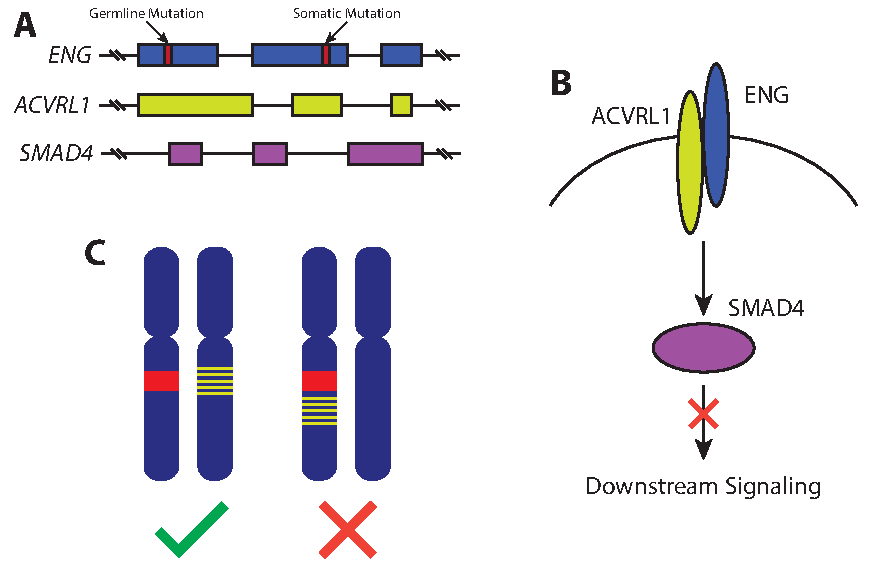
\includegraphics[width=5in]{HHT_TwoHitExpectations}
\end{center}
\caption[Expectations of a Two-Hit Model of HHT] {\textbf{Expectations of a Two-Hit Model of HHT.}\\ The expectations of a two-hit model are: (\textbf{A}) a germline and somatic mutation in the same gene, (\textbf{B}) both the germline and somatic mutations result in loss of function, and (\textbf{C}) that the germline and somatic mutations exist in a \italicize{trans} configuration (i.e. biallelic). }

\label{HHT_TwoHitExpectations}
\end{figure}
%%%%%%%%%%%%%%%%%%%%%%%%%%%%%%

\subsection{Telangiectasia Harmor a Somatic Mutation in \italicize{ENG} or \italicize{ACVRL1}}
We used capture-based library preparations to sequence 19 telangiectasia for the three genes mutated in HHT (\italicize{ENG}, \italicize{ACVRL1}, and \italicize{SMAD4}) and 13 other vascular malformation-related genes (see Methods for identity of genes). The 13 non-HHT vascular malformation genes were chosen with the possibility that they also might harbor somatic mutations, but primarily to serve as control genes, since the two-hit mechanism requires a mutation in the corresponding HHT gene harboring the causal germline mutation.  Somatic mutations in these other genes may or may not contribute to HHT pathogenesis, but absence of a somatic mutation in the casual HHT gene would violate the first expectation of the genetic two-hit mechanism.

In each telangiectasia we identified a pathogenic germline mutation in either \italicize{ENG} or \italicize{ACVRL1}.   Although in most cases the individuals’ germline mutation was already known from clinical diagnostic sequencing, we intentionally remained blinded to this information until after our own sequence analysis of the tissue samples.  In 6003-1, the individual harbors a silent germline mutation which was found by the clinical lab and noted as a variant of unknown significance.  Below we show that this variant is indeed the pathogenic germline variant in this individual.

We used the MuTect2 variant caller to detect variants present in the sequence data. To identify candidate somatic mutations, we removed variants based on several stringent filtering criteria including briefly; intronic or intergenic variants, population frequency $>$0.01\%, $<$0.1\% or $<$5 total supporting reads, low coverage, strand specificity, and low base quality scores. 
To validate or refute the authenticity of each candidate somatic mutation we performed an independent round of amplification using primers flanking each putative variant position for each sample, and sequenced to $>$10000x coverage.   In each tissue sample, the identical somatic variant was re-identified.  Thus, these variants were bona fide somatic mutations existing in the telangiectatic tissue. In total, we identified somatic variants in 9 of 19 telangiectasia; 5 in \italicize{ENG}(NM\_001114753.1 (\italicize{ENG}\_v001)) 4 in \italicize{ACVRL1}(NM\_000020.2 (\italicize{ACVRL1}\_v001)) (Table~\ref{HHT_Table_1}) (Figure~\ref{HHT_Figure_1}) (See Methods). In each case, the somatic mutation was found in the same gene as the pathogenic germline mutation.   Somatic mutations were not found in any of the other 15 genes sequenced, not even in one of the other HHT casual genes.  Importantly, no telangiectasia harbored more than a single somatic mutation. The lack of mutational noise suggests these mutations are pathobiologically significant.  Importantly, all are consistent with strong mutations; five of the variants are small indels resulting in a frameshift, three are in-frame indels, and one is a point mutation 4 bases after an exon-intron boundary that is predicted to impact RNA splicing.

%%%%%%%%%%%%%%%%%%%%%%%%%%%%%%
%				     TABLE 1					%
%%%%%%%%%%%%%%%%%%%%%%%%%%%%%%
\setlength{\rotFPtop}{20pt plus 1fil}
\setlength{\rotFPbot}{-5pt plus 1fil}
\begin{sidewaystable}[]
\footnotesize
\renewcommand{\arraystretch}{1.2} 
\centering
\caption[Mutations Identified in HHT Telangiectasia]{\textbf{Mutations Identified in HHT Telangiectasia.}}

\begin{tabularx}{\textheight}{c p{3.5cm} p{3.5cm} XXX}
\toprule
\textbf{Sample} & \textbf{Germline Mutation} & \textbf{Somatic Mutation} & \textbf{Discovery Reads}\textsuperscript{a} & \textbf{Validation Reads}\textsuperscript{a} & \textbf{Constitutional Reads}\textsuperscript{a} \\
\midrule
6001-1  & \textit{ENG} \newline c.1080\_1083del & \textit{ENG} \newline c.293\_304del & 33/1318 (2.5\%)  & 1067/100268 (1.1\%) & 0/26462 (0\%) \\\hline
6001-3 & same as above & \textit{ENG} \newline c.1195\_1196delAGfsX2 & 5/1080 (0.46\%) & 723/115963 (0.62\%) & 0/24357 (0\%) \\\hline
6001-7 & same as above & \textit{ENG} \newline c.1237\_1238insCAfsX7 & 27/5127 (0.53\%) & 341/115570 (0.30\%)  & 0/23066 (0\%) \\\hline
6001-8 & same as above & \textit{ENG} \newline c.578delCinsTGCG p.T193MR & 111/4845 (2.3\%) & 1142/142572 (0.80\%) & 0/21315 (0\%) \\\hline
6001-10 & same as above & \textit{ENG} \newline c.205delGfsX6 & 33/3389 (1.0\%)  & 3575/326894 (1.1\%)  & 0/22098 (0\%)b \\\hline
6001-* & same as above & NF & & & \\\hline
6002-1 & \textit{ACVRL1} \newline c.1451G\textgreater{}A  p.R484Q & \textit{ACVRL1} \newline c.349delGinsTTfsX52 & 20/2217 (0.90\%) & 309/24018 (1.3\%) & 0/65818 (0\%) \\\hline
6002-2 & same as above & \textit{ACVRL1} \newline c.1378-3\_1402del19ins9 & 26/1649 (1.6\%) & 3189/202550 (1.6\%) & 6/155855 (0.0038\%) \\\hline
6003-1 & \textit{ACVRL1} \newline c.474A\textgreater{}T p.G158G  & \textit{ACVRL1} \newline c.625+4A\textgreater{}T & 101/3392 (3.0\%) & 372/16303 (2.3\%) & 2/38924 (0.0051\%) \\\hline
6004-1 & \textit{ACVRL1} \newline c.1232G\textgreater{}A p.R411Q & NF &	 & & \\\hline
6004-2 & same as above & NF & & & \\\hline
6005-1 & \textit{ACVRL1} \newline c.1232G\textgreater{}A p.R411Q & \textit{ACVRL1} \newline c.1206delCfsX12 & 133/1664 (8.0\%) & 2671/189690 (1.4\%) & N/A \\
\bottomrule
\multicolumn{6}{l}{*Eight additional telangiectasia from patient 6001 with no identified somatic mutation} \\
\multicolumn{6}{l}{For multiple telangiectasia collected from one individual the sample ID is listed as (Patient\#)-(Telangiectasia\#, NF = None Found)} \\
\multicolumn{6}{l}{\textsuperscript{a}Allele frequency in other telangiectasia from 6001} \\
\label{HHT_Table_1}
\end{tabularx}

\end{sidewaystable}
%%%%%%%%%%%%%%%%%%%%%%%%%%%%%%



%%%%%%%%%%%%%%%%%%%%%%%%%%%%%%
%				     FIGURE 1					%
%%%%%%%%%%%%%%%%%%%%%%%%%%%%%%
\begin{figure}[tbp!]
\begin{center}
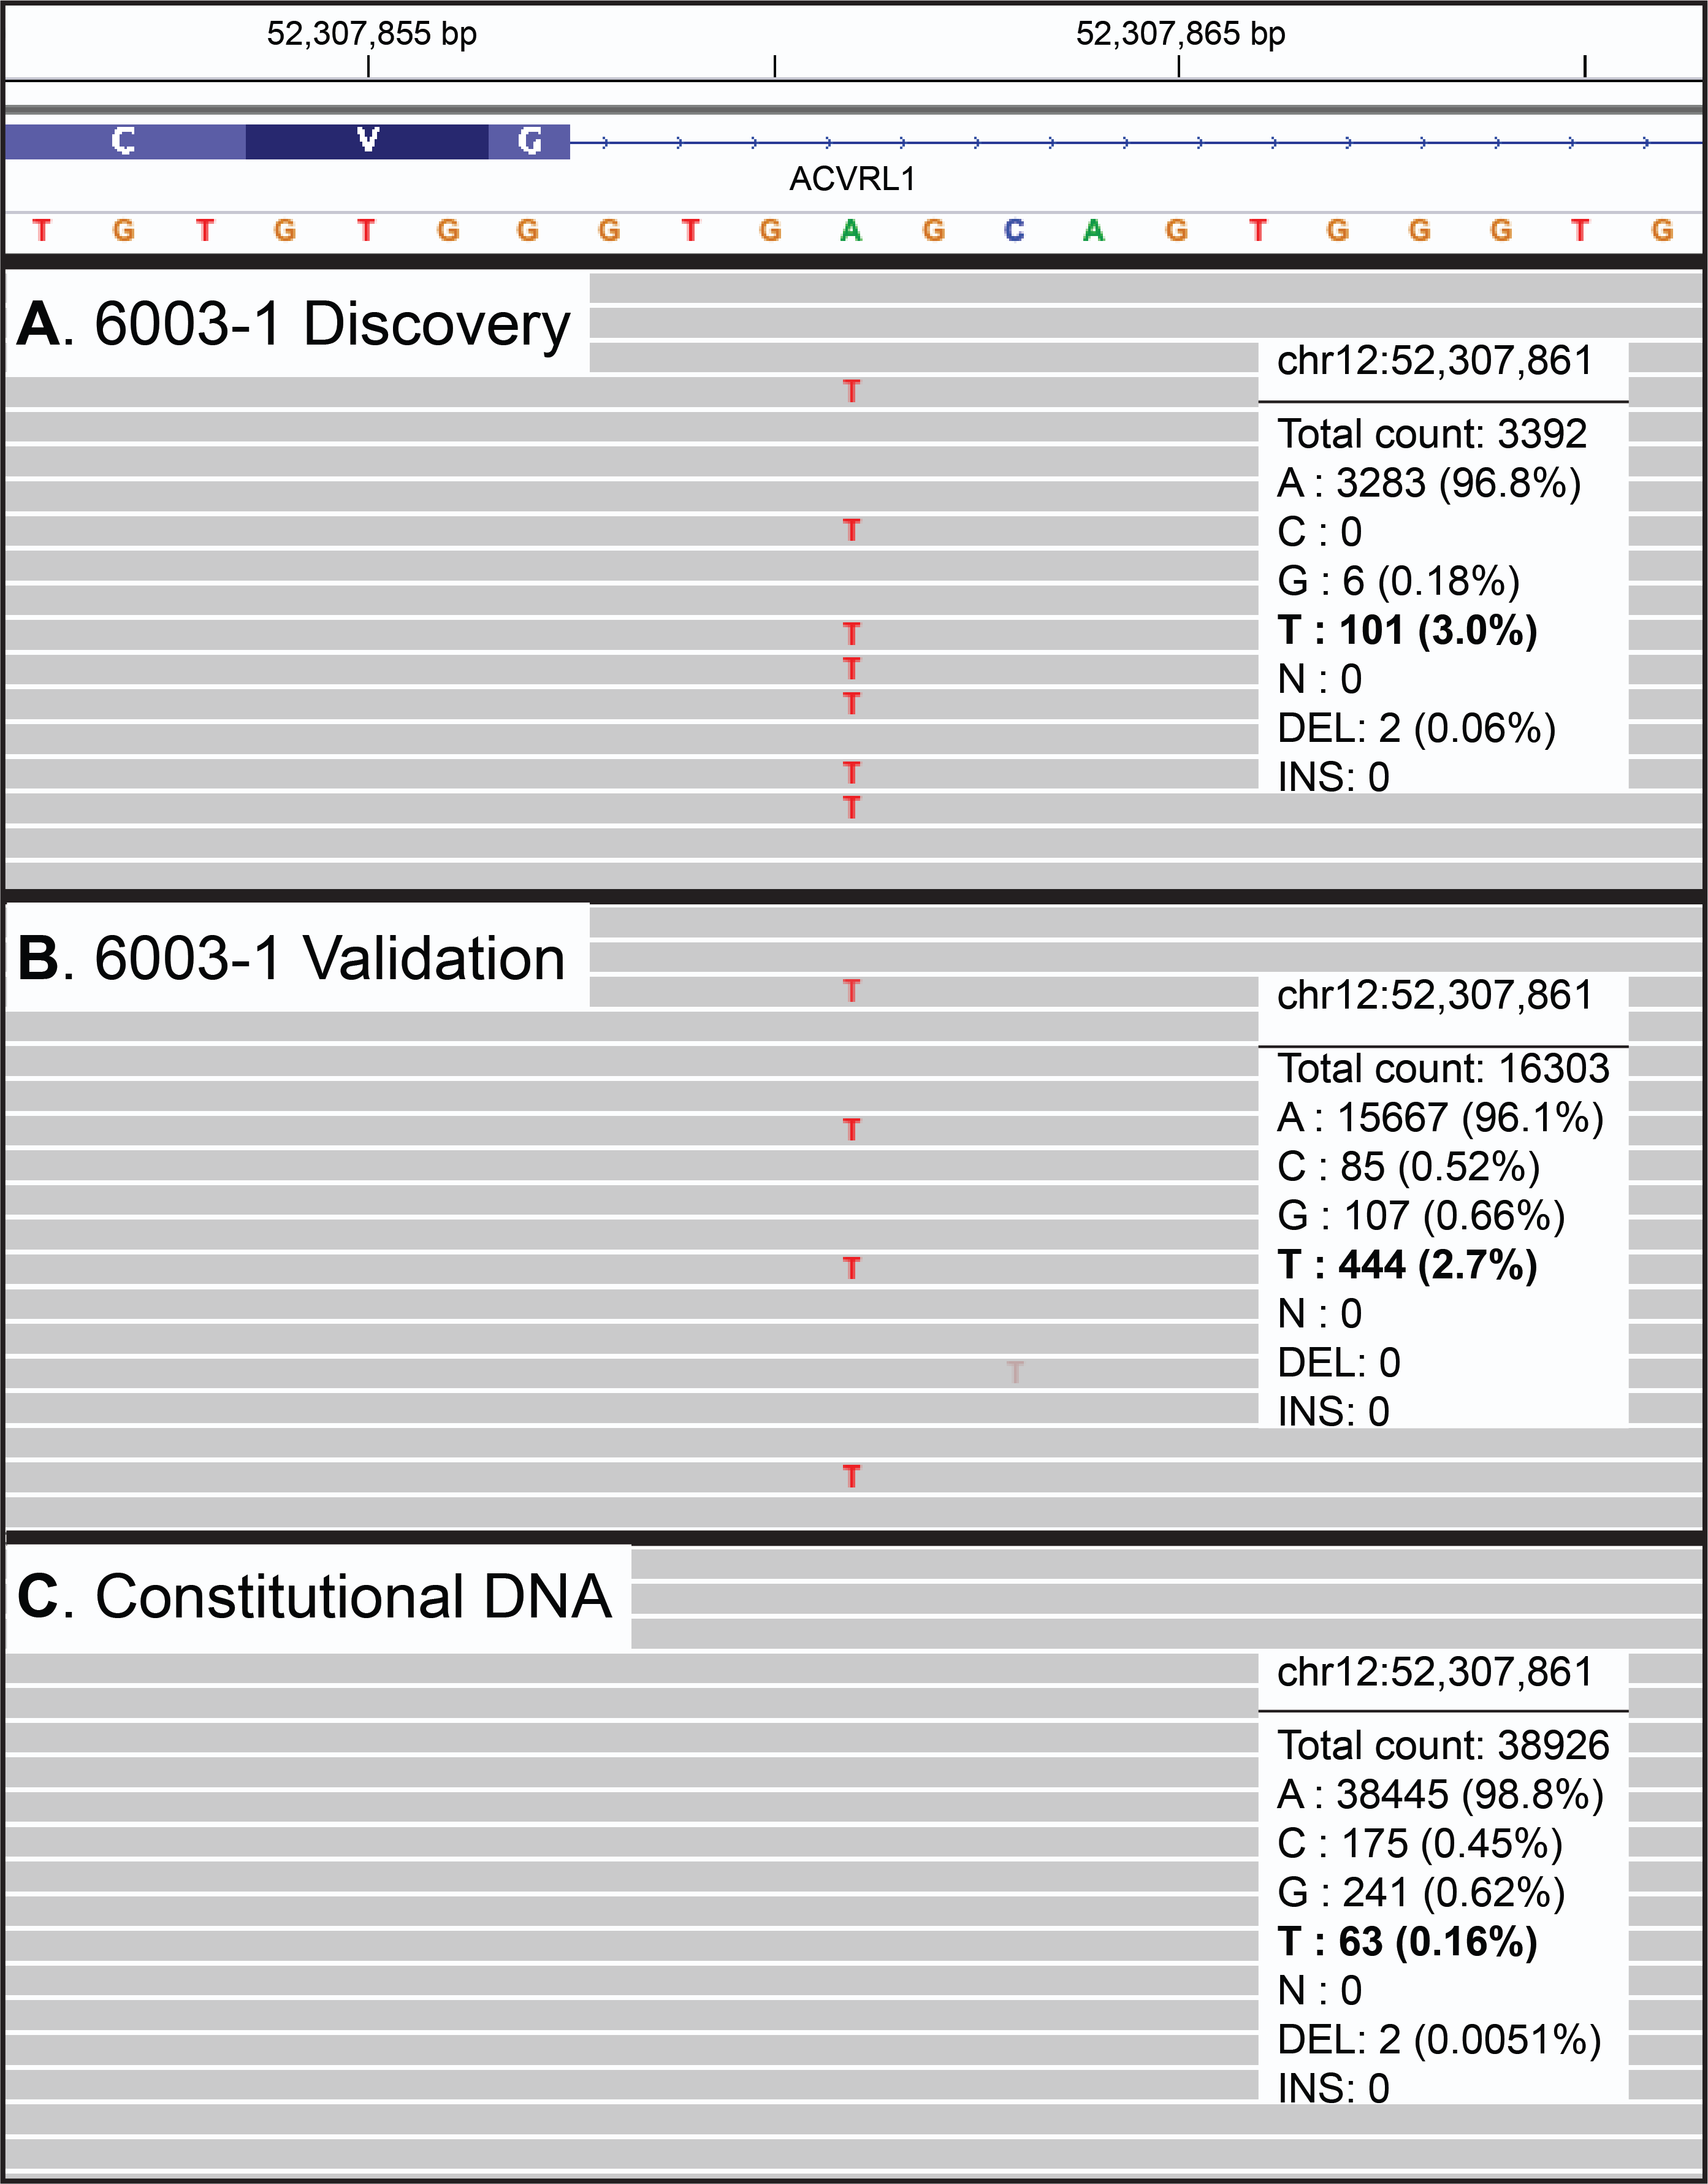
\includegraphics[width=5in]{HHT_Fig1}
\end{center}
\caption[Low Frequency Somatic Mutations Detected in Telangiectasia] {\textbf{Low Frequency Somatic Mutations Detected in Telangiectasia.}\\ Visualization with IGV of next-generation sequencing data for one representative sample with a somatic mutation in \italicize{ACVRL1}. The somatic mutation in 6003-1, an A$>$T point mutation, is present at low frequency in DNA from telangiectatic tissue used for (\textbf{A}) discovery (capture-based sequencing) and (\textbf{B}) validation (amplicon-based sequencing). The mutation is below the level of sequencing noise in (\textbf{C}) constitutional DNA (amplicon-based sequencing) confirming the mutation is somatic.}

\label{HHT_Figure_1}
\end{figure}
%%%%%%%%%%%%%%%%%%%%%%%%%%%%%%

Although these variants fall well below the 50\% allele frequency expected for germline variants, it is formally possible that these variants exist constitutionally as very rare, somatic mosaic variation in the individual.  We next investigated whether these somatic mutations were present in constitutional DNA from the individual. A source of constitutional DNA (saliva) was available for three of the nine mutation-positive samples, and in each we find that the somatic mutation was completely absent or present at a level no higher than technical sequencing noise in that sample (see Methods).  Saliva was not available for 6001, but we obtained and sequenced DNA from multiple telangiectasia collected from this same individual. This enabled us to determine whether any of the five somatic mutations that we identified in individual samples was present in tissue of near identical pathobiology from the same individual; compared with saliva as a control, this is a more powerful test for somatic mosaicism. We found that the somatic mutations identified in five of the telangiectasia for which we identified a mutation were entirely absent in all other telangiectasia from this same individual. Finally, Sample 6005-1 is a single archived FFPE telangiectasia and no source of constitutional DNA is available. In total, we found that 9 of 19 telangiectasia harbor a somatic mutation specifically in the same gene as a pathogenic germline mutation and that these mutations are not present constitutionally. The presence of somatic mutations in telangiectasia fulfills the 1st expectation of the genetic two-hit mechanism. 

\subsection{Somatic and Germline Mutations are Biallelic}
The 2nd expectation of the genetic two-hit mechanism is that the somatic and germline mutations are biallelic; such that the somatic mutation occurs on the wild-type allele of the affected gene, in trans with the germline mutation. To determine if the mutations are biallelic we examined whether they were arranged in a cis or trans configuration by sequencing amplicons that cover the nucleotide positions of both somatic and germline mutations in a single molecule. The amplicons were sequenced with either short-read (Illumina) or long-read (PacBio) chemistry, depending on the amplicon size, in order to generate reads that would span the two mutations. In contrast to traditional Sanger sequencing which measures the population average at each position, both Illumina and PacBio chemistries output sequences of single DNA molecules.  In total we generated mutation-spanning reads for 7 telangiectasia, each with more than 100 reads that contained the somatic mutation. From these mutation-spanning reads we established that $>$95\% of reads with the somatic mutation possessed the wild type allele at the position of the germline mutation, showing that all 7 mutation pairs are in trans configuration (Table~\ref{HHT_Table_2}) (Figure~\ref{HHT_Figure_2}A-B). Any two variants in a chromosome must be arranged in cis or trans with an equal probability of either arrangement. Considering this, our observation that 7/7 mutation pairs are arranged in trans corresponds to a p-value of 0.008 demonstrating significant bias towards a trans configuration. These data show that the somatic and germline mutations are biallelic, fulfilling the 2nd expectation of the genetic two-hit mechanism.

%%%%%%%%%%%%%%%%%%%%%%%%%%%%%%
%				     TABLE 2					%
%%%%%%%%%%%%%%%%%%%%%%%%%%%%%%
\begin{table}[]
\footnotesize
\renewcommand{\arraystretch}{1.4} 
\centering
\caption[Phase of Somatic and Germline Mutation Pairs]{\textbf{Phase of Somatic and Germline Mutation Pairs.}}

\begin{tabularx}{0.75\linewidth}{lllll}
\multicolumn{5}{l}{} \\
\toprule
\textbf{Sample} & \textbf{Total Reads} & \textbf{Trans Reads} & \textbf{Cis Reads} & \textbf{P-value} \\
\midrule
6001-1	& N/A	& N/A						& N/A		& N/A \\\hline
6001-3	& 112	& 112 (100\%)\textsuperscript{a}	& 0 (0\%)		& $1.9\times10^{-34}$ \\\hline
6001-7	& 155	& 153 (98.7\%)\textsuperscript{a}	& 2 (1.3\%)	& $2.6\times10^{-43}$ \\\hline
6001-8	& 593	& 590 (99.5\%)\textsuperscript{a}	& 3 (0.5\%)	& $1.0\times10^{-171}$ \\\hline
6001-10	& N/A	& N/A						& N/A		& N/A \\\hline
6002-1	& 125	& 120 (96.0\%)\textsuperscript{a}	& 5 (4.0\%)	& $5.5\times10^{-30}$ \\\hline
6002-2	& 3189	& 3160 (99.0\%)\textsuperscript{bc}	& 29 (1.0\%)	& $4.2\times10^{-890}$ \\\hline
6003-1	& 372	& 364 (97.8\%)\textsuperscript{bc}	& 6 (1.4\%)	& $1.4\times10^{-99}$ \\\hline
6005-1	& 2671	& 2653 (99.3\%)\textsuperscript{bc}	& 18 (0.7\%)	& $6.3\times10^{-759}$ \\

\bottomrule
\multicolumn{5}{l}{\textsuperscript{a}Reads generated with PacBio long-read chemistry)} \\
\multicolumn{5}{l}{\textsuperscript{b}Reads generated with Illumina short-read chemistry} \\
\multicolumn{5}{l}{\textsuperscript{c}These reads were also used for validation shown in Table~\ref{HHT_Table_1}} \\
\label{HHT_Table_2}
\end{tabularx}

\end{table}
%%%%%%%%%%%%%%%%%%%%%%%%%%%%%%



%%%%%%%%%%%%%%%%%%%%%%%%%%%%%%
%				     FIGURE 2					%
%%%%%%%%%%%%%%%%%%%%%%%%%%%%%%
\begin{figure}[tbp!]
\begin{center}
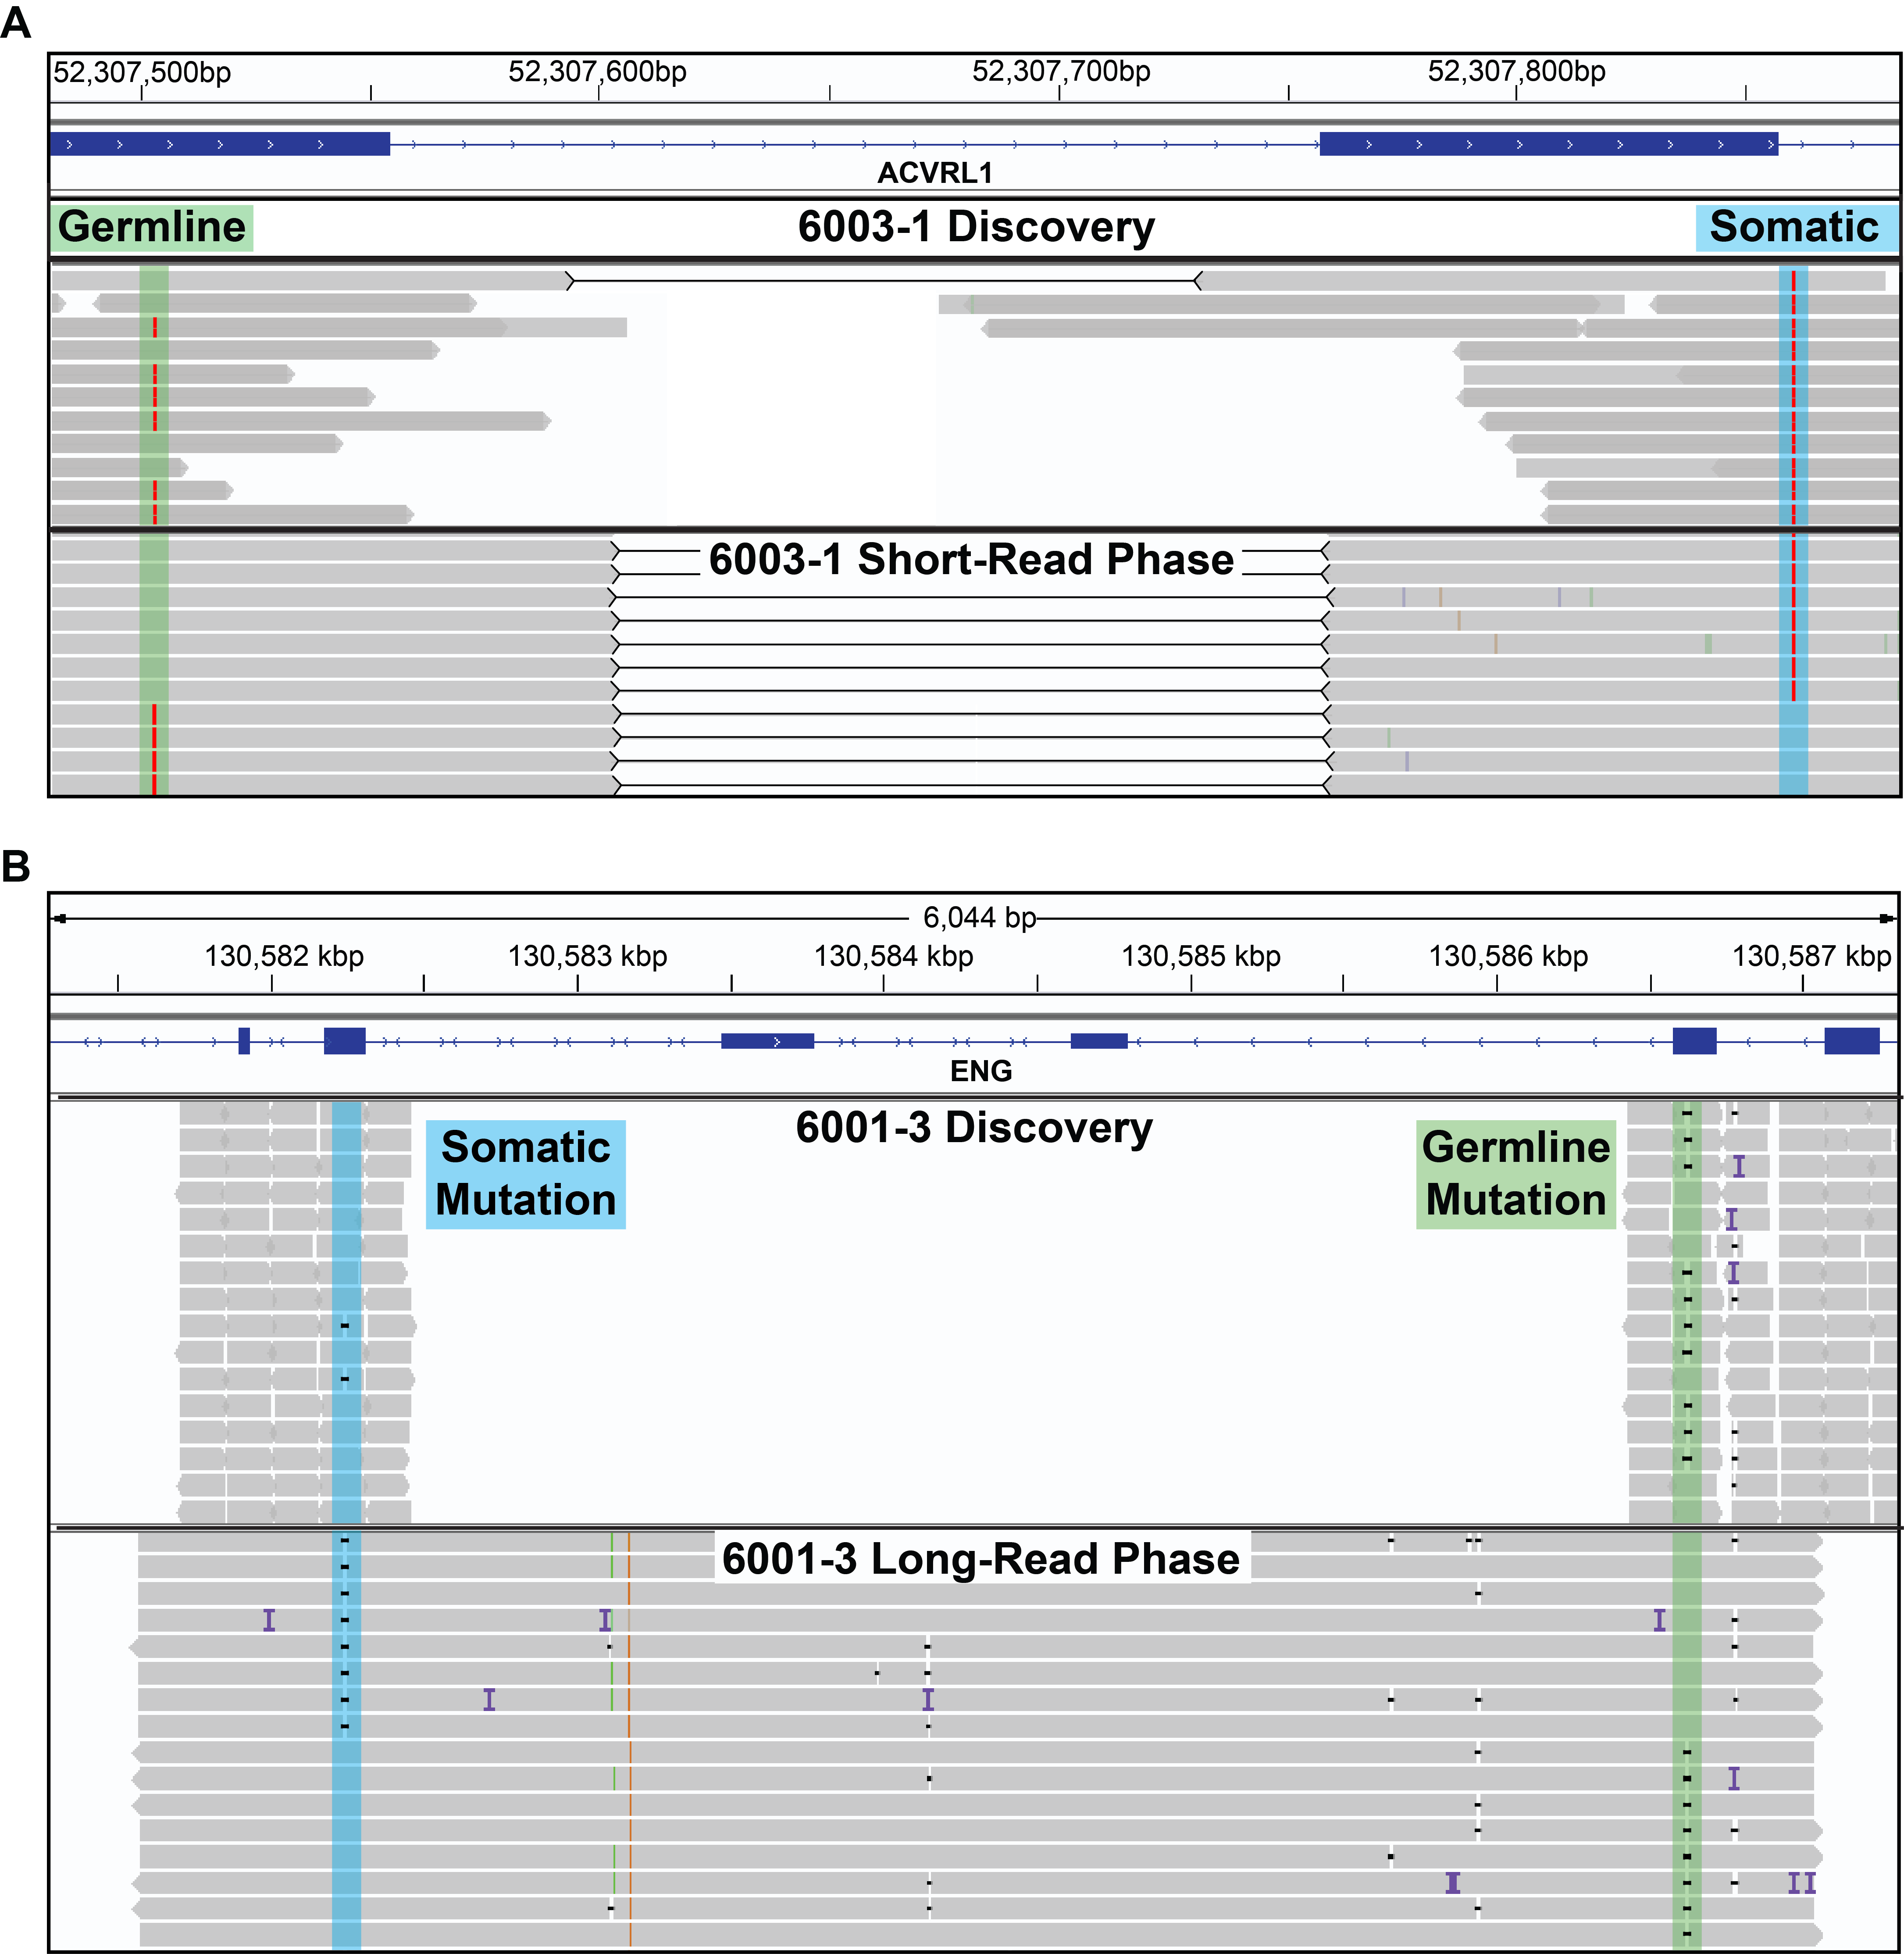
\includegraphics[width=0.9\textwidth]{HHT_Fig2}
\end{center}

\caption[Establishing Phase of Germline and Somatic Mutations]{\textbf{Establishing Phase of Germline and Somatic Mutations.}\\IGV visualization of two samples showing both methods of establishing phase. Each panel shows reads from the initial discovery sequencing and the reads used to establish phase. \textbf{A}, Somatic and germline mutations in 6003-1 are both A$>$T point mutations and highlighted by the blue and green regions respectively. Since the distance between these mutations is relatively small (357bp) phase was established using Illumina short-reads (also used for validation). Black lines between reads denote read pairs, showing that both reads originate from a single molecule of DNA. Each molecule with the somatic mutation contains the wild-type allele at the germline mutation position proving the mutations are biallelic. \textbf{B}, Somatic and germline mutations in 6001-3, both small deletions. The genomic distance between these mutations is 4377bp. In long reads that span the two mutations, each read with the somatic mutation contains the wild-type allele at the position of the germline mutation.}

\label{HHT_Figure_2}
\end{figure}
%%%%%%%%%%%%%%%%%%%%%%%%%%%%%%

\subsection{Mutations are Consistent with Homozygous Loss of Function}
The 3rd expectation of the genetic two-hit mechanism is that the biallelic somatic and germline variants both result in loss of function. Due to the functional studies and extensive allelic series of mutations in each of the HHT genes, HHT is known to be caused by loss of function mutations.   The germline mutation in 4 of the 5 individuals in this study has been identified previously in an individual with HHT and are reported in ClinVar (6001:VCV000213214.2, 6002:VCV000212796.2, 6004/6005:VCV000008243.2).   There are also several publications supporting the pathogenicity of these mutations \citep{johnson1995, bossler2006, gallione1998, ricard2010, olivieri2007}.  These are all therefore bona fide loss of function mutations.  The germline mutation in 6003-1, a silent mutation in \italicize{ACVRL1} exon 4, has been identified before in an individual with HHT, however it was classified as a variant of unknown significance (VUS). We used the in silico tool Human Splicing Finder 3.1 \citep{desmet2009} to analyze this variant and found that it was predicted to both disrupt an exonic splice enhancer and create an internal splice donor site, potentially activating a cryptic splice site. Based on this prediction, we extracted RNA from peripheral blood leukocytes of 6003 and a control individual and performed RT-PCR to examine the splicing of \italicize{ACVRL1} transcripts. RNA from 6003 shows a new splice variant that is not present in control wild-type RNA (Figure~\ref{HHT_Figure_3}B). As predicted by the Splice Finder program, the aberrant transcript is spliced precisely at the internal splice donor created by the mutation. The resulting transcript is missing the portion of exon 4 downstream of the germline mutation and skips exon 5 resulting in the in-frame deletion of 52 amino acids (Figure~\ref{HHT_Figure_3}D-E). This deleted region contains several codons with known pathogenic missense mutations, suggesting that the 52 amino acid deletion would likely also result in loss of function. It is possible that the skipping of exon 5 is due to alternative splicing observed only in peripheral blood leukocytes, rather than a result of the mutation. If exon 5 is retained, the mutation would then generate a protein lacking 17 amino acid residues from exon 4 but then be frameshifted for the remainder of the transcript.  With this evidence, all of the identified germline mutations meet the American College of Medical Genetics (ACMG) criteria for pathogenic mutations \citep{richards2015}, fulfilling the first half of the 3rd expectation of the genetic two-hit mechanism.  

%%%%%%%%%%%%%%%%%%%%%%%%%%%%%%
%				     FIGURE 3					%
%%%%%%%%%%%%%%%%%%%%%%%%%%%%%%
\begin{figure}[tbp!]
\begin{center}
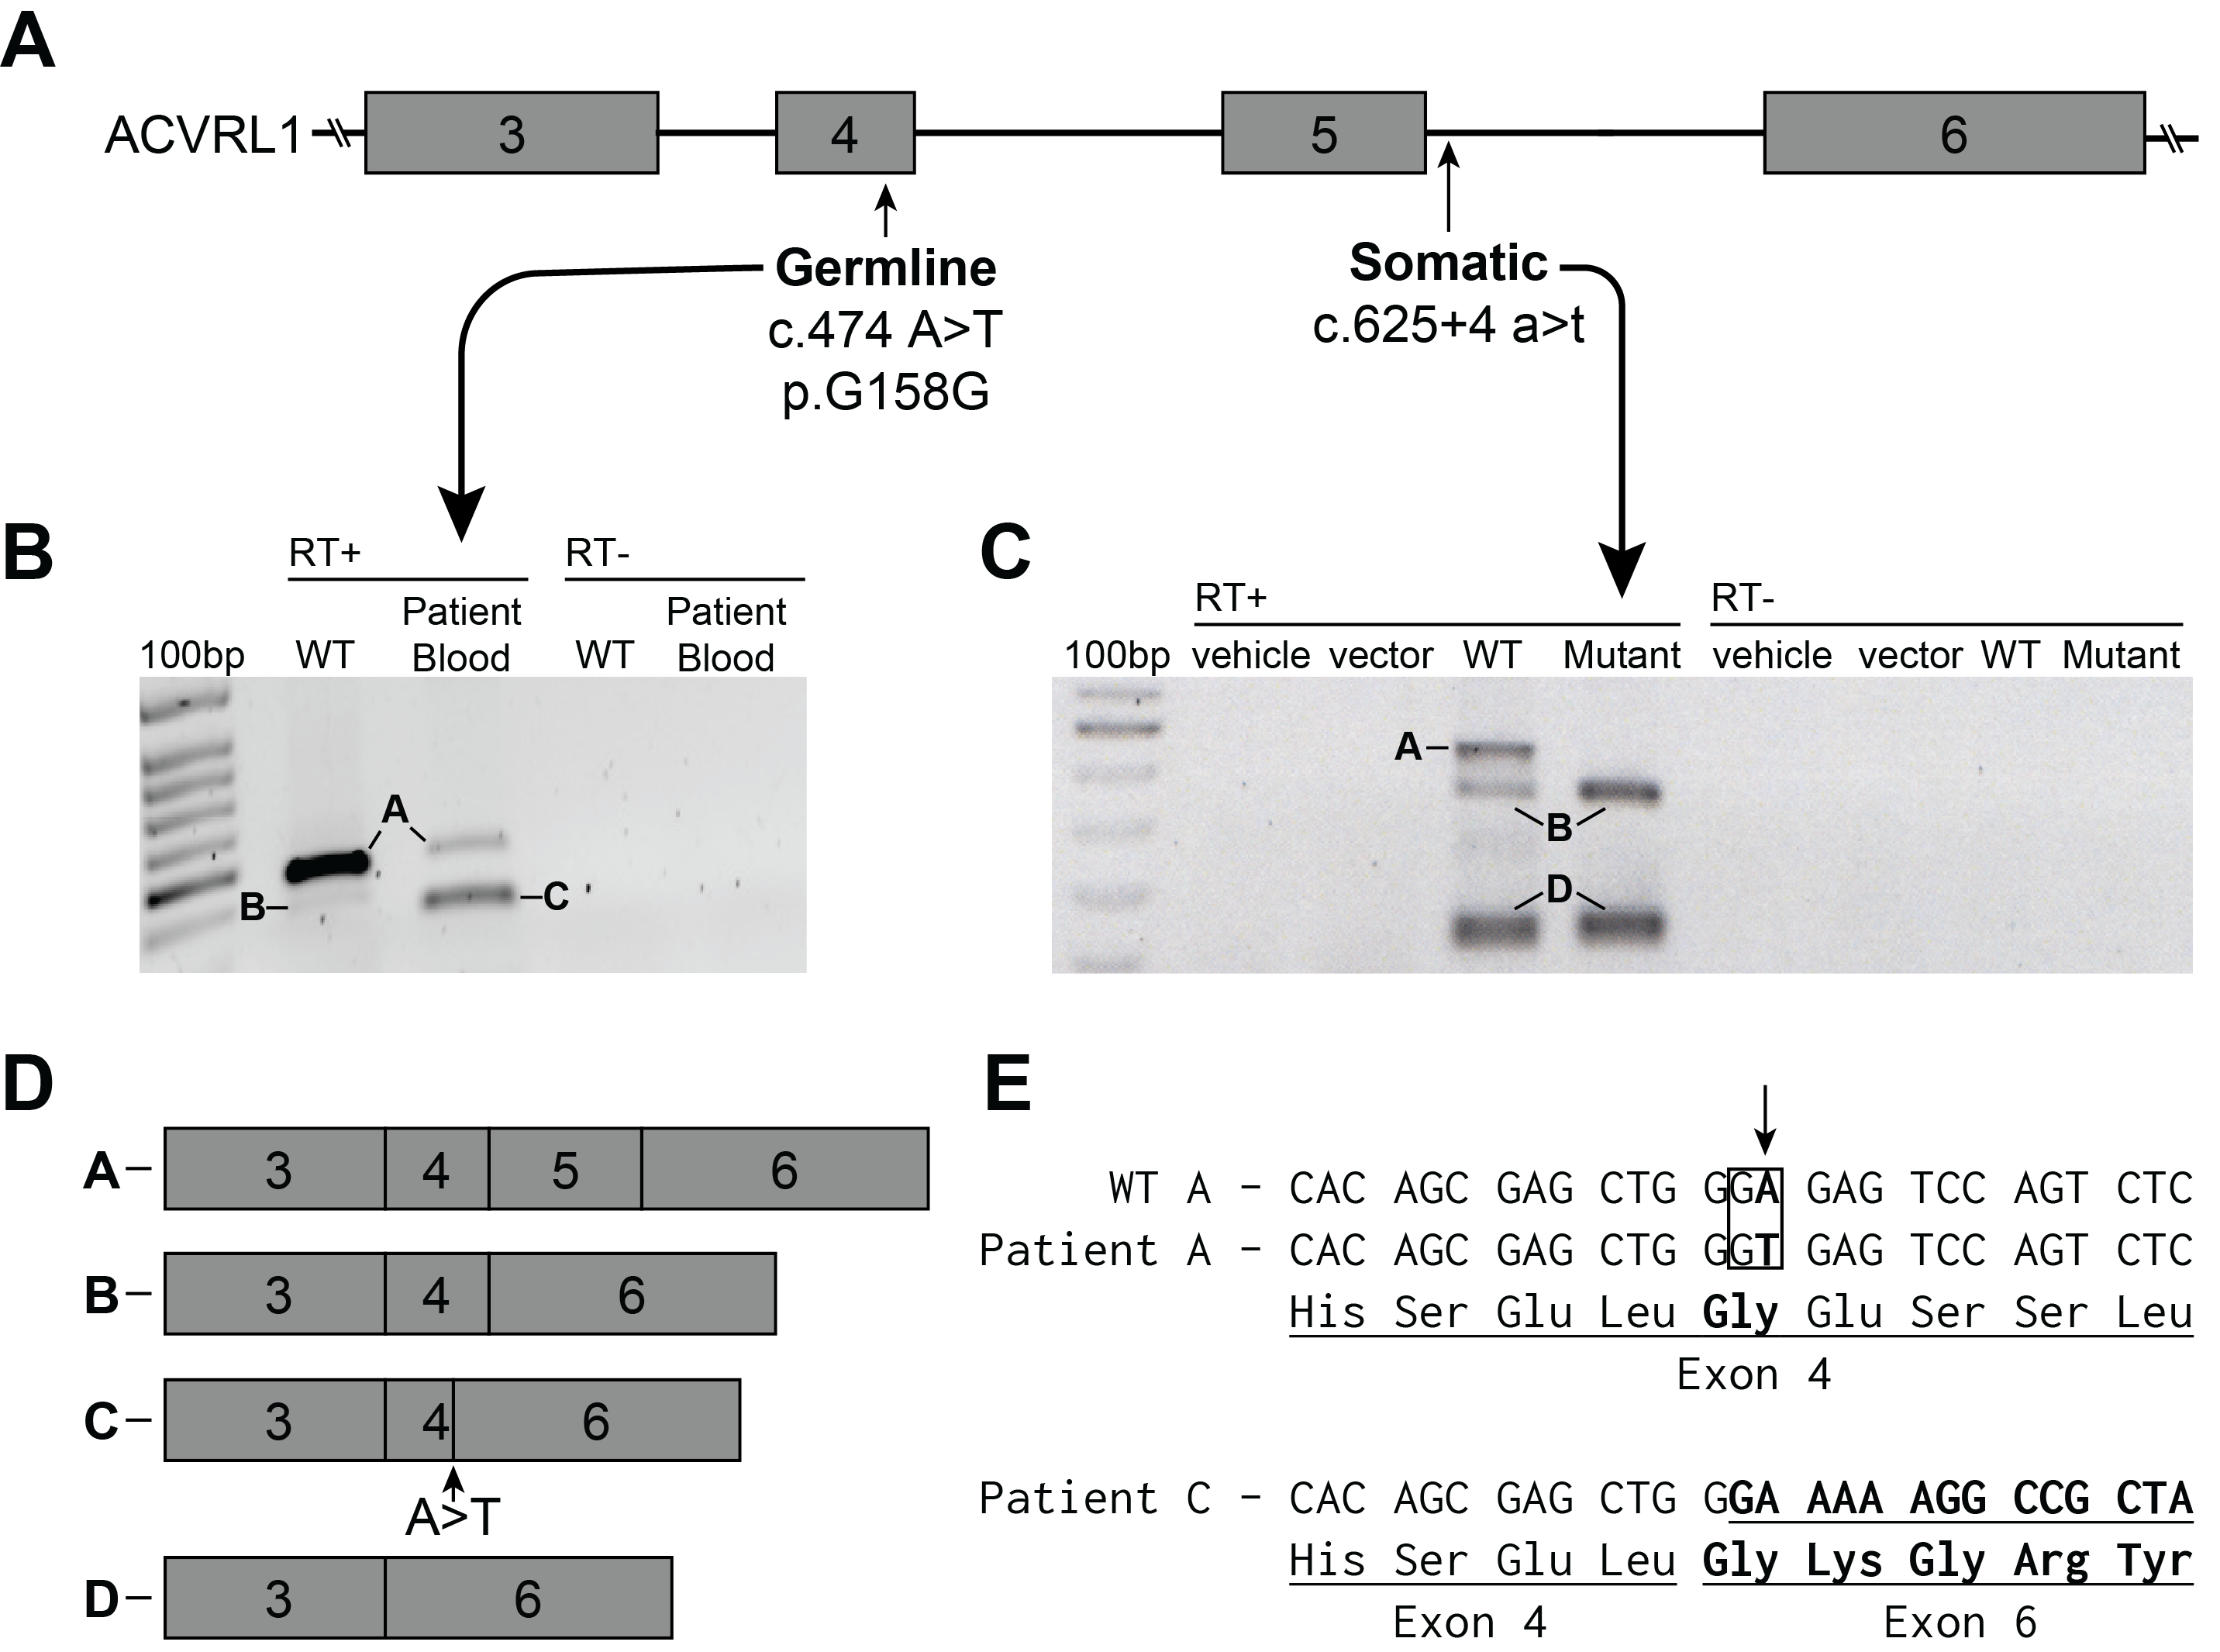
\includegraphics[width=0.95\textwidth]{HHT_Fig3}
\end{center}

\caption[Mutations in \italicize{ACVRL1} Disrupt Splicing]{\textbf{Mutations in \italicize{ACVRL1} Disrupt Splicing.} \\ \textbf{A}, The gene structure of \italicize{ACVRL1} exons 3--6 marked with the location of the germline and somatic mutations found in 6003-1. \textbf{B}, RT-PCR showing \italicize{ACVRL1} transcripts from peripheral blood leukocytes taken from wild-type (WT) and peripheral blood leukocytes containing the germline mutation. The labeled bands were excised and sequenced. Full length transcript (Band A) is present in both the control and leukocytes from 6003 although the level in leukocytes from 6003 is greatly reduced.  Band B in the control contains complete exons 3, 4 and 6.  This splice variant has been seen previously and differs from band C in 6003 which splices from the newly created splice donor site within exon 4 directly to exon 6. \textbf{C}, As the somatic mutation is only present in 3.0\% of reads it would be challenging to detect misspliced RNA from the biopsied tissue. Therefore, we inserted wild-type and mutant sequence of \italicize{ACVRL1} into an in vitro splicing vector, pSPL3-\italicize{ACVRL1}, and used RT-PCR to visualize the impact of the mutation on splicing. Only WT band A shows the full-length transcript containing exon 5; there is no corresponding full-length transcript from the plasmid containing the somatic mutation. \textbf{D}, Exon structure of \italicize{ACVRL1} transcripts determined by sequencing the excised bands. \textbf{E}, Sequence of DNA showing the nature of the germline mutation. In \italicize{ACVRL1} transcripts containing the germline mutation, exon 4 is shortened due to the activation of a cryptic splice site. }

\label{HHT_Figure_3}
\end{figure}
%%%%%%%%%%%%%%%%%%%%%%%%%%%%%%

In contrast to the germline mutation, many of which have been previously identified, the somatic mutations we identified are all novel. The ACMG guidelines for establishing pathogenicity are not applicable to somatic variants, however several lines of evidence support that all of the somatic mutations result in loss of function. Five of the nine somatic mutations result in a frameshift; all resulting in premature termination codons which would generate transcripts susceptible to nonsense-mediated decay. Frameshift mutations in \italicize{ENG} or \italicize{ACVRL1} are the most common mechanism for loss of function leading to HHT. Based on this, the 5 somatic frameshift mutations likely result in loss of function. Other than frameshift mutations, the other 4 somatic mutations we identified consisted of 3 in-frame deletions and 1 intronic mutation predicted to impact splicing. These 4 mutations are not present in the genome aggregation database (gnomAD) showing that the population allele frequency of these variants is extremely low or zero. For the somatic in-frame deletion mutation found in 6001-8, there are two reports of different in-frame deletions with overlap at this position which are known to cause HHT, suggesting that the somatic deletion in 6001-8 is likely to result in loss of function. The somatic mutations in 6001-1 and 6002-2 also result in in-frame deletions, which delete 4 and 7 amino acids respectively. Comparing the crystal structures of \italicize{ENG} and \italicize{ACVRL1} we determined that the somatic mutations in 6001-1 and 6002-2 delete portions of a beta strand and helix respectively, potentially impacting protein folding (Table~\ref{HHT_Table_3}). The in silico tool PROVEAN was used to predict how the protein would tolerate these deletions.   The threshold of -2.5 or lower (more negative) is considered a deleterious change. The scores for 6001-8, 6001-1, and 6002-2 were -6.106, -14.903, and -25.903 respectively, strongly suggesting that all three are deleterious. The remaining somatic mutation is intronic, and occurs 4 nucleotides from the exon-intron boundary. We used Human Splicing Finder 3.1 to predict the effect of this variant on splicing, and found that it is likely to disrupt the donor site. This prediction was confirmed by RT-PCR using an in vitro splicing construct which revealed that the somatic mutation prevents the formation of full-length \italicize{ACVRL1} transcripts (Figure~\ref{HHT_Figure_3}C). In summary we present evidence supporting that the biallelic germline and somatic mutations all likely result in loss of function, fulfilling the 3rd expectation of the genetic two-hit mechanism. 

%%%%%%%%%%%%%%%%%%%%%%%%%%%%%%
%				     TABLE 3					%
%%%%%%%%%%%%%%%%%%%%%%%%%%%%%%
\begin{table}[]
\footnotesize
\renewcommand{\arraystretch}{1.7} 
\centering
\caption[Predicted Consequences of Germline and Somatic Mutations]{\textbf{Predicted Consequences of Germline and Somatic Mutations.}}

\begin{tabularx}{\textwidth}{l p{4.4cm} X}
\multicolumn{3}{l}{} \\
\toprule
\textbf{Sample} & \textbf{Germline Mutation} & \textbf{Somatic Mutation} \\
\midrule
6001-1 & Frameshift: PVS1 \newline 6 supporting publications &In-Frame Deletion (-4 residues) \newline PROVEAN: Deleterious (-14.903) \newline deletes region in $\beta$-sheet \newline gnomAD AF: 0 \\\hline
6001-3 & same as above & Frameshift \newline common ENG LOF mechanism, expect NMD \\\hline
6001-7 & same as above & Frameshift \newline common ENG LOF mechanism, expect NMD \\\hline
6001-8 & same as above & In-Frame Delins (-1 +2 residues) \newline 2 pathogenic in-frame indels overlapping this codon \citep{shovlin1997, argyriou2006} \newline PROVEAN: Deleterious (-6.106) \newline gnomAD AF: 0 \\\hline
6001-10 & same as above & Frameshift \newline common ENG LOF mechanism, expect NMD \\\hline
6002-2 & same as above & In-Frame Delins (-7 +1 residues) \newline PROVEAN: Deleterious (-25.903) \newline deletes region in $\alpha$-helix \newline gnomAD AF: 0 \\\hline
6003-1 & Cryptic Splice Site: PS3 \newline in silico predicted to activate cryptic site \newline in vitro evidence (Figure~\ref{HHT_Figure_3}) & Splice Site \newline in silico predicted to disrupt donor site \newline gnomAD AF: 0 \\\hline
6005-1 & Missense: PS1 \newline 16 supporting publications & Frameshift \newline common \italicize{ACVRL1} LOF mechanism, expect NMD \\
\bottomrule
\multicolumn{3}{l}{\scriptsize{AF = Allele Frequency; NMD = Nonsense Mediated Decay}} \\
\multicolumn{3}{l}{\scriptsize{Germline variant classification according to ACMG guidelines \citep{richards2015}}} \\
\multicolumn{3}{l}{\scriptsize{PVS1 = Very strong evidence for pathogenicity; PS1-4 = Strong evidence}} \\
\multicolumn{3}{l}{\scriptsize{PROVEAN scores below -2.5 are predicted deleterious}} \\
\label{HHT_Table_3}
\end{tabularx}

\end{table}
%%%%%%%%%%%%%%%%%%%%%%%%%%%%%%

\subsection{Telangiectasia from the Same Individual Harbor Unique Somatic Mutations}
We next sought to determine whether mutant cells in different telangiectasia derive from a somatic mutation in a common ancestor cell, or whether the mutant cell population in each telangiectasia derives from an independent somatic mutation event. To test this, we examined the somatic mutations present in multiple telangiectasia from single individuals. In 6001, for which we had obtained 13 different telangiectasia, we identified a somatic mutation in 5 telangiectasia tissue samples.  In each case the somatic mutation in each telangiectasia was unique. Likewise, for 6002, for which we had two telangiectasia, we identified a unique somatic mutation in each (Figure~\ref{HHT_Figure_4}). These results are consistent with independent mutation events rather than the somatic mutation occurring in a progenitor cell or clonality due to a metastasis from a single initial lesion. 

%%%%%%%%%%%%%%%%%%%%%%%%%%%%%%
%				     FIGURE 4					%
%%%%%%%%%%%%%%%%%%%%%%%%%%%%%%
\begin{sidewaysfigure}[tbp!]
\begin{center}
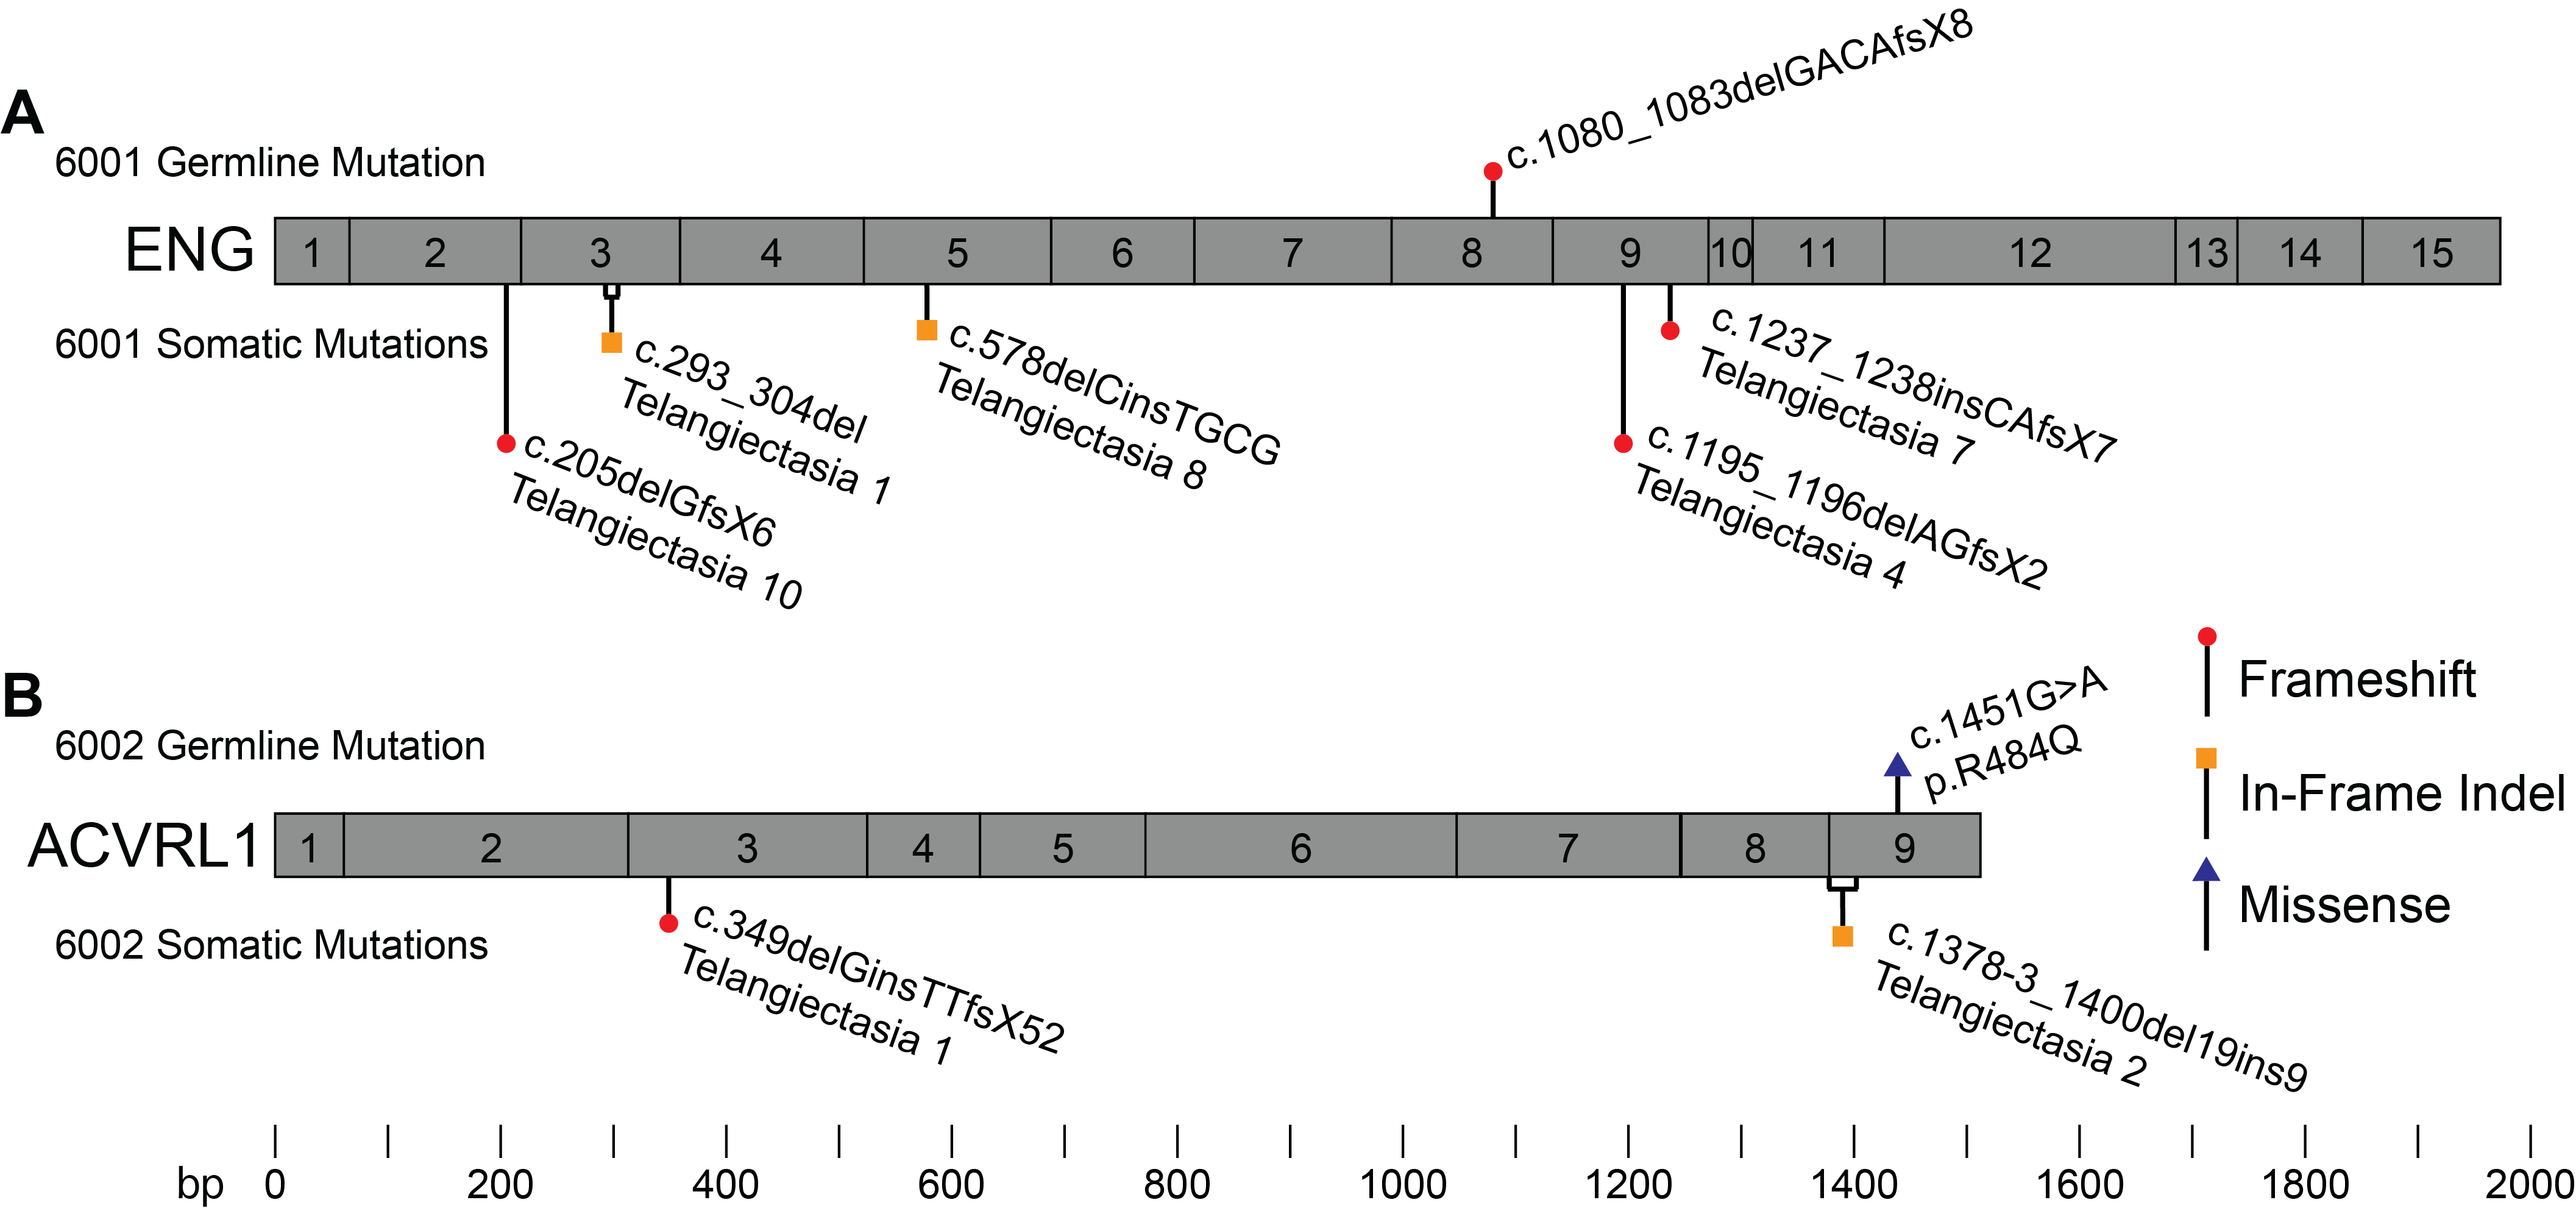
\includegraphics[width=0.9\textwidth]{HHT_Fig4}
\end{center}

\caption[Each Telangiectasia is Seeded by a Unique Somatic Mutation]{\textbf{Each Telangiectasia is Seeded by a Unique Somatic Mutation.} \\ Schematic representation of exons in \italicize{ENG} and \italicize{ACVRL1} with germline and somatic mutations identified in (\textbf{A}) 5 telangiectasia collected from 6001 and (\textbf{B}) 2 telangiectasia collected from 6002. In each panel the common germline mutation is listed above the gene and somatic mutations in each telangiectasia below the gene. Gene structure and mutation position are drawn to scale. }

\label{HHT_Figure_4}
\end{sidewaysfigure}
%%%%%%%%%%%%%%%%%%%%%%%%%%%%%%

\section{Discussion}
\subsection{Evidence for a Genetic Two-Hit Mechanism}
In this study we present strong evidence that vascular malformations associated with HHT, specifically, cutaneous telangiectasia, follow a genetic two-hit mechanism of pathogenesis (Figure~\ref{HHT_TwoHitModel}). HHT is also associated with arteriovenous malformations in lung, liver, brain and the gastrointestinal tract, but these tissues are not available for prospective collection.  We postulate that the visceral, deeper vascular malformations that occur in HHT also follow this two-hit mechanism.  

%%%%%%%%%%%%%%%%%%%%%%%%%%%%%%
%				     FIGURE 5					%
%%%%%%%%%%%%%%%%%%%%%%%%%%%%%%
\begin{figure}[tbp!]
\begin{center}
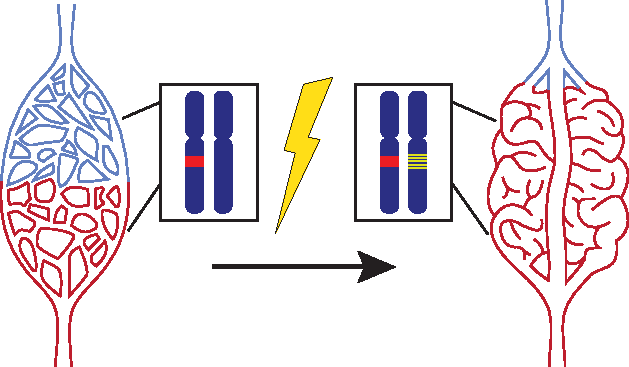
\includegraphics[width=5in]{HHT_TwoHitModel}
\end{center}

\caption[Two-Hit Model of HHT Pathogenesis]{\textbf{Two-Hit Model of HHT Pathogenesis.} \\  Each endothelial cell in someone with HHT is heterozygous for either \italicize{ENG}, \italicize{ACVRL1}, or \italicize{SMAD4} (red bar). A somatic mutation (yellow stripes) occurs in the wild type allele of the same gene with the inherited mutation to induce the formation of an AVM.}

\label{HHT_TwoHitModel}
\end{figure}
%%%%%%%%%%%%%%%%%%%%%%%%%%%%%%

The two-hit hypothesis for HHT pathogenesis has persisted for decades without evidence, but these low frequency somatic mutations are challenging to identify using traditional sequencing methods.  The only published study to address this topic employed immunohistochemical staining in an attempt to identify endothelial cells lacking staining in the lining of HHT-related arteriovenous malformations \citep{bourdeau2000}. However, the absence of staining as a proxy for the gain of a mutation could be difficult to discover, especially if only a fraction of a cells would exhibit this lack of signal.

Using next-generation sequencing with unique molecular identifiers we successfully identified somatic mutations in multiple telangiectasia from different individuals with HHT.  The somatic mutations we identified were present at frequencies ranging between 0.46\% and 8.0\% in the tissue, with an average of 2.3\%. The low allele frequency is likely a result of two main contributing factors; the presence of normal tissue in the skin biopsy, and somatic mosaicism within the telangiectasia. The telangiectasias in this study were sampled as skin punch biopsies and although some of the surrounding skin tissue was removed before DNA extraction, an undetermined amount of normal tissue invariably remained.  However, after removing the surrounding tissue, the enrichment for the vascular component of the tissue was subjectively greater than the often low somatic mutation allele frequency might suggest. We posit that a second explanation for the low mutant allele frequency is that telangiectasia are mosaic for the somatic mutation. This agrees with existing data from mouse models of HHT showing that induced retinal AVMs are mosaic: consisting of both heterozygous and homozygous null cells \citep{jin2017}. It is also consistent with the heterogeneity seen in Cerebral Cavernous Malformations \citep{detter2018, malinverno2019} and the low mutant allele frequency in somatic mutations of other vascular malformation disorders \citep{alolabi2018, soblet2017, limaye2015, limaye2009, shirley2013, couto2015, luks2015, nikolaev2018, couto2017, akers2009, mcdonald2014}.  Vascular malformations, similar to tumors in cancer, appear to be seeded by somatic mutations; however unlike tumors, vascular malformations do not appear to consist of pure populations of clonally expanded mutant cells, but contain a substantial percentage of unmutated cells.   	

	In addition to the data presented here, the two-hit hypothesis of HHT-related vascular malformations is consistent with observations from mouse models of the disease. Whereas constitutional loss of both copies of \italicize{Eng} or \italicize{Acvrl1} in mice is embryonic lethal, mice heterozygous for constitutional deletion of either gene show extremely mild phenotypes with relatively few, if any, detectable vascular malformations\citep{bourdeau1999, srinivasan2003}. Robust mouse models of HHT that recapitulate vascular malformation phenotypes require the use of Cre-Lox technology to delete both copies of \italicize{ENG} in a temporally controlled (postnatal), cell-type specific (endothelial cells) manner. 
	
	In these mouse models of HHT it is also required that biallelic KO of the HHT gene occur in endothelial cells. Several groups have experimented with expressing Cre recombinase in different vascular-related cell types including pericytes (\italicize{NG2}-Cre), vascular smooth muscle cells (\italicize{Myh11}-Cre), and endothelial cells (\italicize{Scl}-Cre \& \italicize{Pdgfb}-Cre); however, mice only develop vascular malformations when Cre is expressed in endothelial cells \citep{tualchalot2015, choi2014, garridomartin2014, mahmoud2010}. We have attempted to confirm that the somatic mutations we identified in human lesions occur in the endothelium by using laser capture microdissection, however these efforts have been hampered by the small quantity of tissue in telangiectasia biopsies and the difficulty of isolating a single layer of cells by microdissection. This question may be more easily addressed in larger arteriovenous malformations; however, these samples have been thus far inaccessible due to the rarity of their removal in individuals with HHT.
	
\subsection{Necessary, but Not Sufficient}
Interestingly, in addition to the local requirement for loss of both alleles, vascular malformations in this model only develop after injury such as an ear punch, or by VEGF injection \citep{choi2012}. This requirement of an angiogenic stimulus is consistent in mouse models for all HHT genotypes: \italicize{Eng}, \italicize{Acvrl1}, and \italicize{Smad4} \citep{kim2018}. The requirement for knockout of both copies of the gene supports the genetic two-hit mechanism we describe here. In addition, the necessity for an angiogenic stimulus suggests that loss of both copies of the relevant HHT gene is necessary, but not sufficient, for the development of the vascular malformation. 

\subsection{Sensitivity for Detecting Somatic Mutations}
	We might have expected to find somatic mutations in every telangiectasia, however we only found somatic mutations in 9 of the 19 we sequenced. The next-generation sequencing strategy we employ for discovering somatic mutations is extremely sensitive for the detection of point mutations and small indels. However, there are several other types of genetic alterations that would result in biallelic loss of function due to loss of heterozygosity (LOH).  LOH is a common occurrence in many tumors in cancer, and is a predominant mechanism of somatic loss/mutation.  LOH can occur due to a variety of genetic mechanisms: large deletions, chromosome loss, and mitotic recombination. Given the apparent capacity for even a low fraction of somatically mutant cells to initiate the vascular malformation, it follows that the same would be true for LOH-associated mutational events; therefore, these mutations would appear instead as allelic imbalance rather than outright LOH.  But if the level of allelic imbalance is as low as the frequency of somatic mutations we have observed in this study, we might expect linked marker haplotype ratios in the range of 48\% to 52\% at nearby markers; this slight and even trivial imbalance would be difficult if not impossible to detect and validate.  It is also possible that non-genetic mechanisms such as loss of expression due to epigenetic silencing account for biallelic loss of function.  This process, like the LOH associated events, would not be detected by our sequencing strategy; a problem that is only exacerbated by low allele frequency. Thus, it may not be surprising that we identified a somatic mutation in approximately only 9 of the VMs that were sequenced. We postulate it is highly likely that all of the 10 telangiectasia with no identified somatic mutation have biallelic loss by one of these other mechanisms.    
	
\subsection{Mutant Cell Metastasis}
One consequence of the genetic two-hit mechanism that might appear to be improbable is that, if true, a new somatic mutation must occur in every one of the numerous vascular malformations in HHT. For example, some affected individuals have dozens or more visible telangiectasia on the skin and mucocutaneous surfaces alone \citep{gonzalez2019, letteboer2008, plauchu1989}.  An attractive hypothesis to reconcile this conundrum would be if a somatic mutation first occurs in a circulating progenitor cell which then proliferates and seeds the formation of multiple telangiectasia.  There is precedence for this mechanism in another vascular malformation syndrome, Blue Rubber Bleb Nevus syndrome.  These individuals display multiple small vascular lesions which harbor an identical somatic double-mutation in the \italicize{TEK} gene. These vascular lesions appear to be anatomically-dispersed clones arising from an original, dominant, large lesion \citep{soblet2017}. In HHT-related vascular malformations, we report evidence that contradicts this hypothesis: different telangiectasia collected from the same individual harbor different, unique somatic mutations. This observation does not exclude the possibility that circulating cells may in some cases spread telangiectasia, however the data thus far suggests that the primary mechanism is independent somatic mutation events. 

\subsection{Probability of Multiple Somatic Mutations}
The dilemma of the requirement for numerous independent somatic mutation events in a single gene can be resolved with a probabilistic argument. Considering the size of the human genome (3.23 $\times$ $10^9$ bp), the probability that a random somatic mutation occurs in the coding sequence of \italicize{ENG} (3201 bp) in trans (50\% likelihood) with a pathogenic \italicize{ENG} germline mutation is $\sim$0.00005\%. Compounding this value with empirical evidence that single cells have anywhere from 100 to 1500 somatic mutations per cell \citep{milholland2017, lodato2015, losardo2017}, and an estimate that 5.66\% of exonic somatic mutations result in LOF \citep{milholland2017}; we calculate a conservative estimate that 0.00028\% of cell have biallelic LOF \italicize{ENG} mutations. An adult human has at least 6 $\times$ $10^{11}$ endothelial cells \citep{sender2016}, therefore we estimate that an individual with HHT and a germline mutation in \italicize{ENG} has biallelic LOF \italicize{ENG} mutations in $\sim$1.5 million endothelial cells. It is clear that each cell with \italicize{ENG} biallelic LOF does not result in vascular malformation as individuals with HHT have at most hundreds, not millions, of telangiectasia. This disparity is consistent with the idea that telangiectasia only develop under very specific conditions: likely that the somatic mutation must occur in a specific type of vascular bed, in an endothelial cell, and must be followed by local angiogenic stimulus.  

\subsection{Two-Hit Mechanism for \italicize{SMAD4} \& JP-HHT}
Our samples consisted of telangiectasia from individuals with HHT from a single HHT Centre of Excellence.  This cohort had germline mutations in either \italicize{ENG} or \italicize{ACVRL1}, and somatic mutations were identified in telangiectasia from both genotypes. Mutations in \italicize{SMAD4} cause the combined syndrome HHT and Juvenile Polyposis (JP-HHT) , however individuals with \italicize{SMAD4} mutations only account for $\sim$2\% of HHT cases \citep{gallione2004}. Unfortunately, no individuals with JP-HHT were present in our cohort, but we believe it is likely that JP-HHT-related telangiectasia follow an identical genetic two-hit mechanism, resulting from somatic mutations in \italicize{SMAD4}. 

\subsection{Compound Heterozygosity}
As HHT is caused by germline mutations in any one of 3 genes, an interesting question is whether the compound effect of a LOF mutation in two different HHT genes could drive pathogenesis (e.g. a germline mutation in \italicize{ENG} and a somatic mutation in \italicize{ACVRL1}). However, thus far all of the somatic mutations we identified in HHT-related telangiectasia occur in the same gene as that harboring the germline mutation.   This human genetic data is consistent with the observation that mice with combined deficiency for one allele each of \italicize{Acvrl1} and \italicize{Eng} are fertile, viable and are not teeming with vascular malformations \citep{eleftheriou2016} (Srinivasan and Marchuk, unpublished), as might be expected if trans-heterozygosity of mutations in these two HHT-genes could initiate vascular malformation development.
	
\subsection{Therapeutic Potential}	
A genetic two-hit mechanism for HHT pathogenesis has therapeutic implications. Certain efforts to develop therapies for HHT assume a model of haploinsufficiency of the relevant HHT gene.  These strategies attempt to increase the amount of the affected gene product by increasing the level of transcript/protein arising from the wild-type allele \citep{ruizllorente2017}. We show here that some fraction of cells within the malformation do not possess a wild-type allele.  Even if expression in surrounding heterozygous cells could be increased, the null cells would remain devoid of protein, suggesting that this avenue of therapy may be ineffective.  By contrast, a more effective strategy may be gene replacement, reintroducing a fully wild-type allele into the mutated cells \citep{seki2003}, as this would simultaneously provide an extra copy of the gene to both the heterozygous and null cells.   This strategy is particularly attractive as it might inhibit new VM formation by adding back a second wild-type copy of the mutated gene.


\section{Methods}
\subsubsection{Sample Collection}
Individuals were enrolled in the study after giving informed consent (approved by either the St. Michael’s Hospital IRB committee or the Duke University Health System IRB Committee).  Diagnosis of HHT was based on identification of a pathogenic germline mutation, or by exhibiting at least three of the four symptoms as per the Cura\c{c}ao criteria (Supp Table 1) \citep{shovlin2000}.
Telangiectasia were resected using a 3mm punch biopsy, after local anesthesia (1\% xylocaine with epinephrine), with standard aseptic technique.  Sample 6005-1 was immediately formalin fixed (10\% formalin) and paraffin embedded (FFPE), and then shipped at room temperature.  All other samples were immediately frozen at -80 Celsius, and then shipped on dry ice.  Saliva samples were obtained using Oragene DNA saliva kits at the time of tissue collection. Blood from individual 6003 was obtained during a subsequent visit, shipped at room temperature, and immediately used for RNA extraction. 

\subsubsection{DNA and RNA Extraction}
DNA from telangiectasia samples was extracted using the DNeasy Blood and Tissue Kit (Qiagen). DNA from FFPE sample 6005-1 was extracted using QIAamp DNA FFPE Tissue Kit (Qiagen). Genomic DNA and RNA were extracted from peripheral blood leukocytes from individual 6003 and from a non-HHT control individual using the Gentra PureGene Blood Kit (Qiagen) and TRIzol Reagent (Invitrogen) extraction protocols, respectively, as per the manufacturers’ directions. 

\subsubsection{Targeted Sequencing}
To enable the detection of somatic mutations in telangiectasia we used a next generation sequencing strategy. Somatic mutations involved in the pathogenesis of other vascular malformation diseases such as cerebral cavernous malformations often have a low allele frequency due to somatic mosaicism in the malformation. Somatic mosaicism is also present in retinal AVMs from mouse models of HHT suggesting that low allele frequency may be a confounder when identifying somatic variants in telangiectasia. In addition, the telangiectasia samples collected for this study consist of bulk biopsied tissue which have not been enriched for any particular cell type. Considering these potential sources of normal (non-mutant) cell contamination, we sequenced telangiectasia to $>$1000x coverage and incorporated a unique molecular identifier to enable the detection of variants as low as 0.1\% allele frequency.
Eighteen fresh-frozen samples and one FFPE sample were sequenced using a custom Agilent SureSelect panel covering 16 genes implicated in various vascular malformation disorders: \italicize{ENG}, \italicize{ACVRL1}, \italicize{SMAD4}, \italicize{BRAF}, \italicize{CCM2}, \italicize{FLT1}, \italicize{FLT4}, \italicize{GNAQ}, \italicize{KDR}, \italicize{KRAS}, \italicize{KRIT1}, \italicize{MAP2K1}, \italicize{NRAS}, \italicize{PDCD10}, \italicize{PIK3CA}, and \italicize{PTEN}. Though \italicize{GDF2} variants have been identified in an HHT-like phenotype, these cases are extremely rare. Moreover, mutations in \italicize{GDF2} have not been identified in any individual at the Toronto HHT Centre for Excellence therefore \italicize{GDF2} was not included in the panel. To ensure the generation of high-quality sequencing libraries, the Agilent NGS FFPE QC Kit was used to determine the extent of DNA degradation in the FFPE sample. Samples with $\Delta$Cq values $>$2 were excluded from the study as per manufacturer recommendation. Sequencing libraries were generated using the Agilent SureSelect XT HS Kit. Samples were then pooled and sequenced on an iSeq 100 (Illumina) with paired-end 150bp reads. Across all samples, target regions were sequenced to a mean depth of 2803x with 78\% of the target region at $>$1000x and 96\% of the target region at $>$100x. 

\subsubsection{Mutation Detection}
Sequencing data was processed and analyzed using a custom pipeline based on the GATK best practices for somatic short variant discovery. Briefly, after analyzing the raw data with fastQC to ensure high quality data, the adapter sequences were trimmed from reads using bbduk, reads were aligned to the hg19 human reference genome using bowtie2, duplicates were removed based on UMI sequence using fgbio, variants were called using MuTect2 in tumor-only mode, and variants were annotated using snpSift. The resulting variant call file (VCF) was filtered through several steps to identify somatic mutations. To identify variants that may change the protein sequence or impact splicing, we selected for variants that occur within exons or within 10bp of an exon. From this set, we removed variants that are present in the population at $>$0.01\% frequency by comparing to 3 databases (dbSNP, 1000 Genomes project, and the Exome Aggregation Consortium [ExAC]); as these variants are more common than the frequency of HHT (1--5 in 10000) \citep{grosse2014}. We removed any variants present in $<$0.02\% of sequence reads, as this is the reported technical limit of detection for the SureSelect XT technology. We also removed variants in regions with $<$100x coverage, variants with $<$5 supporting reads, variants that were strand specific, and variants where $<$50\% of alternative bases had a quality score $>$30 ($>$Q30). 
	Candidate somatic variants identified in the targeted sequencing data were then validated by sequencing amplicons generated during a second, independent round of PCR amplification. We designed primers for each sample to specifically amplify the position of the somatic mutation and 100--200bp of flanking sequence. When possible, the primers were designed such that they would capture the position of both the germline and somatic mutations within a single amplicon. Each primer was synthesized with the following Illumina flow cell adapter sequences such that the amplicons could be easily indexed and sequenced: 
	\\
	\\For: 5’-TCGTCGGCAGCGTCAGATGTGTATAAGAGACAG‐[primer]-3’
	\\Rev: 5’-GTCTCGTGGGCTCGGAGATGTGTATAAGAGACAG‐[primer]-3’
	\\\\
	Amplicons were prepared from telangiectasia DNA and constitutional DNA if available (Supp Table 1) using two rounds of PCR. The first round of PCR was 25 cycles and served to amplify the target region from genomic DNA. Amplicons from the first round were purified using AMPure XP beads (Beckman Coulter) and used for a second round of PCR using 8 cycles to attach a sample index using the Nextera XT Index Kit. Amplicons from the second round were purified, pooled, and sequenced on an iSeq 100 with 150bp paired-end reads to a depth of $>$10000x. The frequency of the somatic mutation in telangiectasia and constitutional DNA was determined using custom scripts, excluding bases $<$Q15. 
	As these amplicons were sequenced in the same run, it is possible for a low level of index misassignment causing switching of reads between samples. This could cause some reads from telangiectasia to be assigned as constitutional reads and vice versa. To estimate the rate of index misassignment, we examined pairs of samples that target different genomic locations and quantified the proportion of misassigned reads between these samples. Based on this we estimate that the rate of misassignment is 0.2--0.8\%, relative to the sample of origin. For example, if one sample has a somatic mutation with a frequency of 1\% and was sequenced to 100000x coverage, then 2--8 reads containing the somatic mutation would be misassigned to each of the other samples in the pool.

\subsubsection{Establishing Phase}
To establish the phase of the somatic and germline mutations we used either short-read sequencing with Illumina chemistry, or long-read sequencing with PacBio chemistry depending on the distance between the two mutations. For mutations $<$500bp apart, we generated amplicons during the validation process that cover the positions of both the somatic and germline mutations. These amplicons were sequenced on an iSeq 100 as described above. 
	For mutations $>$500bp we designed primers such that the resulting amplicon would cover the position of both the germline and somatic mutations for each sample. Each primer was synthesized with the PacBio ‘universal tag’ as follows to enable indexing and sequencing: 
	\\
	\\For: 5'-/5AmMC6/GCAGTCGAACATGTAGCTGACTCAGGTCAC-[primer]-3'
	\\Rev: 5'-/5AmMC6/TGGATCACTTGTGCAAGCATCACATCGTAG-[primer]-3'
	\\\\
	We generated amplicons spanning the somatic and germline mutations using the LongAmp Taq DNA Polymerase Kit as per manufacturer instructions. These amplicons were purified with AMPure XP beads and used for a second round of PCR to attach the sample index. This process used no more than 30 cycles of PCR total. These amplicons were pooled and sequenced across one SMRT cell on a PacBio Sequel System. The sequence reads were aligned to the hg19 human genome using Minimap2 in ava-pb mode.
The single molecule resolution of these technologies allowed us to determine how the mutant alleles are arranged; if the mutations are in trans then reads will have either the somatic mutant allele or the germline mutant allele, if the mutations are in cis then reads will have either no mutant alleles or both mutant alleles. In total we generated mutation-spanning reads for 7 telangiectasia, each with $>$100 reads which contained the somatic mutation. The p-values reported for phase status were calculated using a binomial distribution with the null hypothesis that a random mutation has an equal probability of cis or trans configuration with a nearby variant. 
The genomic distance between mutations varied greatly with the closest mutations in sample 6005-1 with 26 bases between mutations, and the most distant in 6001-10 with 18.7 kilobases between mutations. Of the 9 telangiectasia with identified somatic mutations, the distance between mutations in 6002-2, 6003-1, and 6005-1 was small enough to allow for mutation-spanning reads using illumina chemistry (Table. 2). Mutation-spanning reads were generated for 6001-3, 6001-7, 6001-8, and 6002-1 using PacBio chemistry. We were unable to generate amplicons spanning the mutations for 6001-1 and 6001-10. The sequence downstream of the somatic mutation in these telangiectasia contains several repetitive regions which, combined with the genomic distance and limited quantity of input DNA may have contributed to PCR failure. 
One notable confounder in this analysis is the generation of chimeric reads resulting from template switching during PCR. The generation of chimeric reads is known to interfere with amplicon-based haplotype phasing by switching a variant from one strand to another, potentially generating new haplotypes not present in the original sample \citep{laver2016}. In practice, chimeric reads randomize the arrangement of the somatic and germline mutations. The frequency of chimeric arrangements is highly dependent on the distance between mutations and the number of PCR cycles used to make the amplicons. To reduce the number of chimeric reads in our libraries we used no more than 30 cycles for amplification. A previous study reports a chimeric arrangement frequency of 6.5\% for 29 cycles of amplification for mutations 9kbp apart \citep{laver2016}. Chimeric reads may account for the very few discordant reads in some of our samples, as shown in Table~\ref{HHT_Table_2}.  Nonetheless, these were so minor in comparison to the great majority of the reads that phase could be unequivocally determined.

\subsubsection{\italicize{in vitro} Splicing}
A 3.8kb fragment of \italicize{ACVRL1} genomic DNA spanning from 431 bases upstream of exon 3 to 215 bases downstream from exon 8 was amplified and this entire insert was ligated into the MCS of pSPL3, a splicing vector \citep{church1994}.  Clones were sequenced to ensure that no PCR-induced errors were present in the exons and adjacent intronic regions of the insert.  The specific mutation, c.625+4A$>$T, was introduced using site directed mutagenesis and again, clones were sequenced to verify that the only sequence difference was at the intended site. Plasmid DNA from empty vector, wild type (control) vector and mutation-containing vector were transfected into HEK293T cells using Lipofectamine 3000 (ThermoFisher Scientific), incubated for 24 hours, and then the RNA was extracted using TRIzol and Direct-zol RNA miniprep kit (Zymo Research).  

\subsubsection{Reverse-Transcription PCR}
RNA extracted from peripheral blood leukocytes and from transfected cells was used as template for cDNA synthesis using the Maxima H Minus First Strand cDNA kit (ThermoFisher Scientific).  An RT primer in \italicize{ACVRL1} exon 8 was used in the RNA from blood while a vector-specific RT primer was used for the RNA from transfected cells to ensure that only RNA from the transfected vectors was being used as template for cDNA synthesis. cDNA from peripheral blood leukocytes was PCR amplified using primers in exons 3 and 6 while cDNA from the transfected cells was PCR amplified using primers in exons 3 and 8.  PCR reactions were run on 1\% agarose gels, the bands excised and Sanger sequenced. 

\section{Contributions and Acknowledgements}
This chapter is adapted from a study published in AJHG \citep{snellings2019} with the following authors: Daniel A. Snellings, Carol J. Gallione, Dewi S. Clark, Nicholas T. Vozoris, Marie E. Faughnan, and Douglas A. Marchuk. DAS performed all sequencing experiments. CJG performed in vitro splicing experiments. DSC, NTV, and MEF provided tissue samples. DAM and DAS designed experiments. 

We thank all participants and their families who donated samples for this study. We thank Dr. Nicolas Devos and the Duke Sequencing and Genomic Technologies Core for assistance designing experiments and sequencing. This study was supported by U.S. Department of Defense grant (W81XWH-17-1-0429) and a Fondation Leducq Transatlantic Network of Excellence Grant in Neurovascular Disease (17 CVD 03). MEF also received financial support from the Nelson Arthur Hyland Foundation. } % A regular chapter, starts with '\chapter{Title}'
%\chapter{Mutant \italicize{GNAQ} Alleles Produce Distinct Disease Phenotypes}

\section{Premise}
\section{Results}
\section{Discussion}
\section{Methods}

}
%\chapter{\italicize{MAP3K3} Mutations Seed Cerebral Cavernous Malformations}

\section{Premise}
\section{Results}
\section{Discussion}
\section{Methods}}
\chapter{\italicize{PIK3CA} Mutations Fuel Cerebral Cavernous Malformation Growth}
\label{hello}

Enjoy some Lorem Ipsum text!
This should create about two full pages of text so you can verify the
margins are correct (especially if you're doing two-sided).

\section{Lorem Ipsum}
Lorem ipsum dolor sit amet, consectetuer adipiscing elit. Sed vitae leo.
Pellentesque quis nisi id orci consectetuer posuere. Quisque malesuada
rhoncus dui. Vivamus mi. Mauris commodo. Phasellus lacus magna, feugiat ac,
blandit ut, rutrum id, massa. In consectetuer magna vel justo. Cras eu
diam. Nullam tortor turpis, bibendum non, consequat ac, tincidunt non,
nisi. 

Curabitur sagittis dignissim arcu. Pellentesque habitant morbi
tristique senectus et netus et malesuada fames ac turpis egestas.
Vestibulum ullamcorper. Curabitur faucibus euismod nulla. Vivamus sagittis.
Sed fermentum neque a risus vestibulum convallis. Morbi id massa ut arcu
mollis commodo. Aliquam erat volutpat.  Pellentesque fringilla pellentesque
nisi. Morbi tristique ornare libero. Vestibulum turpis sapien, iaculis ut,
cursus non, condimentum in, tortor. Aenean vehicula. Integer egestas
tincidunt erat. Aenean euismod ante vel lectus. Duis ac sapien vel erat
euismod aliquet. Vivamus tempor placerat nibh. Curabitur pharetra, orci
consequat pulvinar ultricies, orci enim tempor augue, non lacinia orci nisl
et nibh. Nunc gravida dictum turpis.  Duis sollicitudin commodo massa. Nam
ac nunc. Fusce sodales posuere velit. Nunc ullamcorper sodales urna. Donec
consectetuer accumsan ante. Morbi feugiat rutrum mauris. Praesent malesuada
auctor est. Pellentesque quis odio non nulla ornare imperdiet. Aliquam
dapibus. Suspendisse posuere, magna in molestie varius, ipsum velit rhoncus
nisi, nec bibendum pede mauris in urna. Morbi purus lectus, molestie quis,
laoreet id, tincidunt at, ligula. 

Praesent sit amet libero id arcu
adipiscing tristique. Quisque libero erat, bibendum nec, malesuada in,
gravida et, urna. Phasellus molestie vulputate nisi. Nullam massa magna,
dignissim ac, accumsan a, scelerisque eu, erat. Nam tellus augue, tempus
nec, molestie sit amet, rhoncus vel, libero. Vestibulum at neque. Aliquam
laoreet tincidunt mi. Ut laoreet ligula ac urna. Nullam nisl pede, posuere
id, dictum a, fermentum vitae, turpis.  Nulla ante mauris, euismod et,
mollis eu, tempor in, quam. 

In pede augue, elementum varius, tincidunt in,
condimentum ut, erat. Etiam vulputate faucibus velit. Aliquam porttitor.
Nam fringilla adipiscing nisi. Sed in magna. Aenean non ante. Aenean
facilisis, nunc sed aliquam porta, magna est aliquam nisi, vitae semper
turpis orci ac dolor. Praesent nec tellus. Cras vulputate rhoncus sem.
Curabitur eu mi. Mauris euismod lacinia nibh. Suspendisse eget sapien et
nunc accumsan elementum.  Nulla dapibus. Donec interdum elit mattis velit
imperdiet aliquet. Mauris feugiat, ante vel faucibus rutrum, eros mauris
sollicitudin neque, ut varius diam ipsum et massa. Nullam non nisi sit amet
tortor rhoncus molestie. Cras consectetuer condimentum ante. Phasellus
fermentum risus fermentum turpis. Mauris dignissim iaculis sem. Fusce nisi
lorem, viverra id, auctor et, scelerisque ut, massa. In hac habitasse
platea dictumst. Vestibulum ante ipsum primis in faucibus orci luctus et
ultrices posuere cubilia Curae; Aliquam pulvinar neque ac dolor.

\section{More nonsense}
Lorem ipsum dolor sit amet, consectetuer adipiscing elit. Sed vitae leo.
Pellentesque quis nisi id orci consectetuer posuere. Quisque malesuada
rhoncus dui. Vivamus mi. Mauris commodo. Phasellus lacus magna, feugiat ac,
blandit ut, rutrum id, massa. In consectetuer magna vel justo. Cras eu
diam. Nullam tortor turpis, bibendum non, consequat ac, tincidunt non,
nisi. 
Curabitur sagittis dignissim arcu. Pellentesque habitant morbi
tristique senectus et netus et malesuada fames ac turpis egestas.

Vestibulum ullamcorper. Curabitur faucibus euismod nulla. Vivamus sagittis.
Sed fermentum neque a risus vestibulum convallis. Morbi id massa ut arcu
mollis commodo. Aliquam erat volutpat.  Pellentesque fringilla pellentesque
nisi. Morbi tristique ornare libero. Vestibulum turpis sapien, iaculis ut,
cursus non, condimentum in, tortor. Aenean vehicula. 

Integer egestas
tincidunt erat. Aenean euismod ante vel lectus. Duis ac sapien vel erat
euismod aliquet. Vivamus tempor placerat nibh. Curabitur pharetra, orci
consequat pulvinar ultricies, orci enim tempor augue, non lacinia orci nisl
et nibh. Nunc gravida dictum turpis.  Duis sollicitudin commodo massa. Nam
ac nunc. Fusce sodales posuere velit. Nunc ullamcorper sodales urna. Donec
consectetuer accumsan ante. Morbi feugiat rutrum mauris. Praesent malesuada
auctor est. 

Pellentesque quis odio non nulla ornare imperdiet. Aliquam
dapibus. Suspendisse posuere, magna in molestie varius, ipsum velit rhoncus
nisi, nec bibendum pede mauris in urna. Morbi purus lectus, molestie quis,
laoreet id, tincidunt at, ligula. 
Praesent sit amet libero id arcu
adipiscing tristique. Quisque libero erat, bibendum nec, malesuada in,
gravida et, urna. Phasellus molestie vulputate nisi. Nullam massa magna,
dignissim ac, accumsan a, scelerisque eu, erat. Nam tellus augue, tempus
nec, molestie sit amet, rhoncus vel, libero. Vestibulum at neque. Aliquam
laoreet tincidunt mi. Ut laoreet ligula ac urna. Nullam nisl pede, posuere
id, dictum a, fermentum vitae, turpis.  Nulla ante mauris, euismod et,
mollis eu, tempor in, quam. 
In pede augue, elementum varius, tincidunt in,
condimentum ut, erat. Etiam vulputate faucibus velit. Aliquam porttitor.

Nam fringilla adipiscing nisi. Sed in magna. Aenean non ante. Aenean
facilisis, nunc sed aliquam porta, magna est aliquam nisi, vitae semper
turpis orci ac dolor. Praesent nec tellus. Cras vulputate rhoncus sem.
Curabitur eu mi. Mauris euismod lacinia nibh. Suspendisse eget sapien et
nunc accumsan elementum.  Nulla dapibus. Donec interdum elit mattis velit
imperdiet aliquet. Mauris feugiat, ante vel faucibus rutrum, eros mauris
sollicitudin neque, ut varius diam ipsum et massa. Nullam non nisi sit amet
tortor rhoncus molestie. Cras consectetuer condimentum ante. Phasellus
fermentum risus fermentum turpis. Mauris dignissim iaculis sem. Fusce nisi
lorem, viverra id, auctor et, scelerisque ut, massa. In hac habitasse
platea dictumst. Vestibulum ante ipsum primis in faucibus orci luctus et
ultrices posuere cubilia Curae; Aliquam pulvinar neque ac dolor.
}
\chapter{Developmental Venous Anomalies Predispose to Malformation}
\label{chap:hht}

\blfootnote{This chapter is adapted from a study published in \italicize{bioR$\chi$iv} (Snellings et al., 2021)}
\clearpage

\section{Premise}
Cerebral cavernous malformations (CCMs) are hemorrhagic neurovascular malformations that may lead to stroke, seizures and other clinical sequelae. CCM disease may be inherited by an autosomal dominant loss of function (LOF) mutation in the genes encoding components of the CCM signaling complex: \italicize{KRIT1} \citep{couteulx1999, sahoo1999}, \italicize{CCM2} \citep{liquori2003}, or \italicize{PDCD10} \citep{bergametti2005}. Solitary sporadic CCM lesions may also occur in the absence of inherited germline mutations in CCM complex genes. Previous studies have established that CCM pathogenesis follows a genetic two-hit model where somatic mutations cause biallelic LOF in \italicize{KRIT1}, \italicize{CCM2}, or \italicize{PDCD10} to initiate lesion formation \citep{akers2009, gault2009, gault2005, mcdonald2014}. Recent studies have found that somatic mutations in \italicize{PIK3CA} and \italicize{MAP3K3} also contribute to CCM pathogenesis \citep{hong2021, ren2021, weng2021}. These discoveries opened new avenues for research and therapeutic development, but they also raised new questions about the roles of somatic mutations in familial versus sporadic lesions. 
	
The presence of multiple somatic mutations in CCMs also helps explain a long-standing mystery: the association between sporadic CCM lesions and developmental venous anomalies (DVA). DVA are the most common vascular malformation present in 6--14\% of the adult population \citep{brinjikji2017, gokce2014, jones2015, linscott2016} with the majority developing prior to the age of 20 \citep{brinjikji2017}.  When assessed by magnetic resonance imaging, an adjacent DVA is identified in 24--32\% of sporadic CCM cases \citep{abdulrauf1999, porter1997, wurm2005}, and an even greater fraction of sporadic CCMs are found to be associated with a DVA at surgery \citep{abdulrauf1999, porter1997}. One study focused on DVA reported an adjacent sporadic CCM in 6.9\% of all DVAs in a general population (116 of 1689) \citep{brinjikji2017}. These studies highlight the association between DVA and sporadic CCM. By contrast, familial CCM lesions have not been associated with DVA \citep{dammann2017}. These combined data suggest that a DVA is not required for CCM formation but may be a predisposing factor in sporadic cases. We hypothesize that DVA are caused by somatic mutations, and that the genetic origin of DVA overlaps that of CCM. In this study we probe the relationship between mutations in \italicize{KRIT1}, \italicize{CCM2}, \italicize{PDCD10}, \italicize{PIK3CA}, and \italicize{MAP3K3} and explore a mechanism by which DVA act as a genetic primer for the genesis of sporadic CCM lesions. 

\section{Results}
\subsection{Mutations in \italicize{MAP3K3} and CCM Genes are Mutually Exclusive}

%%%%%%%%%%%%%%%%%%%%%%%%%%%%%%
%				     FIGURE 1					%
%%%%%%%%%%%%%%%%%%%%%%%%%%%%%%
\begin{figure}[tbh]
\centering
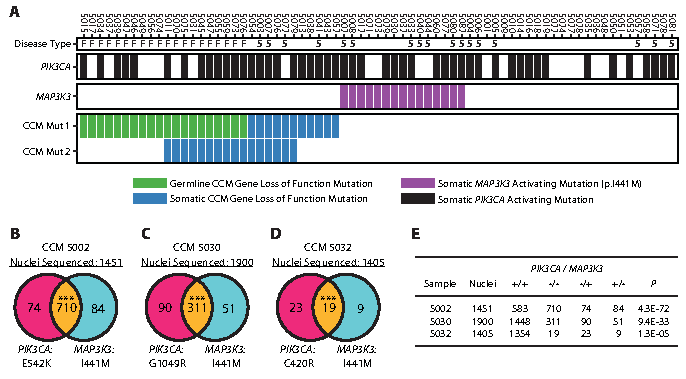
\includegraphics[width=6in]{MAP_discovery}
\caption[\italicize{MAP3K3} Somatic Mutations and Cellular Phase in CCM]{\textbf{Mutations in \italicize{MAP3K3} are Mutually Exclusive with CCM Mutations and Occur in the Same Cells as \italicize{PIK3CA} Mutations.\\} 
\textbf{A.} Mutations present in 71 CCM samples. Disease type denotes whether the sample was familial (F), sporadic (S), or unknown (blank). The presence of somatic mutations in \italicize{PIK3CA} and \italicize{MAP3K3} are denoted by black and purple bars respectively. Germline and somatic mutations (green and blue respectively) in \italicize{KRIT1}, \italicize{CCM2}, or \italicize{PDCD10}, are shown in CCM Mut 1 with the second-hit mutation shown in CCM Mut 2 if present. \textbf{B--D.} Nuclei genotypes determined by snDNA-seq. The left and right circles in each Venn diagram shows the number of nuclei with the \italicize{PIK3CA} or \italicize{MAP3K3} mutations where the overlap shows nuclei harboring both mutations. *** P $<$ 0.0001. \textbf{E.} Summary of data presented in B--D including P values determined by comparing the observed number of double mutant nuclei to the expected value derived from a Poisson distribution as done previously \citep{ren2021}. }

\label{MAP_discovery}
\end{figure}
%%%%%%%%%%%%%%%%%%%%%%%%%%%%%%

To evaluate whether sporadic and familial CCMs have distinct somatic mutation spectra we identified somatic mutations present in 71 CCMs (20 familial CCMs and 51 sporadic/presumed sporadic CCMs). Mutations in \italicize{KRIT1}, \italicize{CCM2}, \italicize{PDCD10}, and \italicize{PIK3CA} were detected by targeted sequencing and/or droplet digital PCR (ddPCR) as previously described \citep{ren2021}. The common gain of function mutation in \italicize{MAP3K3} (hg38 chr17:63691212, NM\_002401.3, c.1323C$>$G; NP\_002392, p.I441M) was detected by ddPCR using a previously published probe set \citep{couto2015}. 

The p.I441M mutation in \italicize{MAP3K3} was identified in 15/51 sporadic CCMs and 0/20 familial CCMs (Figure~\ref{MAP_discovery}A). We also screened for \italicize{MAP3K3} p.I441M in 8 blood samples for which we were previously unable to identify a germline mutation in \italicize{KRIT1}, \italicize{CCM2}, \italicize{PDCD10}. None of the 8 blood samples harbored \italicize{MAP3K3} p.I441M. Notably 11/51 sporadic CCMs harbored at least 1 somatic mutation in \italicize{KRIT1}, \italicize{CCM2}, or \italicize{PDCD10}, however none of these CCMs also had a mutation in \italicize{MAP3K3} indicating that a mutual loss of the CCM complex and gain of function in MEKK3 (the protein product of \italicize{MAP3K3}) are not both required for CCM formation. As the CCM complex is known to be a direct inhibitor of MEKK3 activity \citep{zhou2015, zhou2016}, these data strongly suggest identical functional consequences of these mutations. 
	
The majority of CCM and verrucous venous malformations with a mutation in \italicize{MAP3K3} harbor the p.I441M variant \citep{couto2015, hong2021, weng2021} , however an alternative variant p.Y544H has also been identified in a venous malformation \citep{alqattan2020}. While ddPCR provides superior sensitivity and specificity compared to targeted sequencing, it is restricted to detecting a single mutation per assay. To determine whether other mutations that contribute to CCM pathogenesis---either \italicize{MAP3K3} mutations besides p.I441M, or mutations in yet undiscovered genes---we performed whole-exome sequencing (mean depth 133x) on 8 sporadic CCMs for which no somatic mutations in \italicize{KRIT1}, \italicize{CCM2}, \italicize{PDCD10}, or \italicize{MAP3K3} were found. No additional mutations in \italicize{MAP3K3} were identified and no candidate variants in other genes passed QC filters (see Methods). 

%%%%%%%%%%%%%%%%%%%%%%%%%%%%%%
%				     FIGURE 2					%
%%%%%%%%%%%%%%%%%%%%%%%%%%%%%%
\begin{figure}[!ht]
\centering
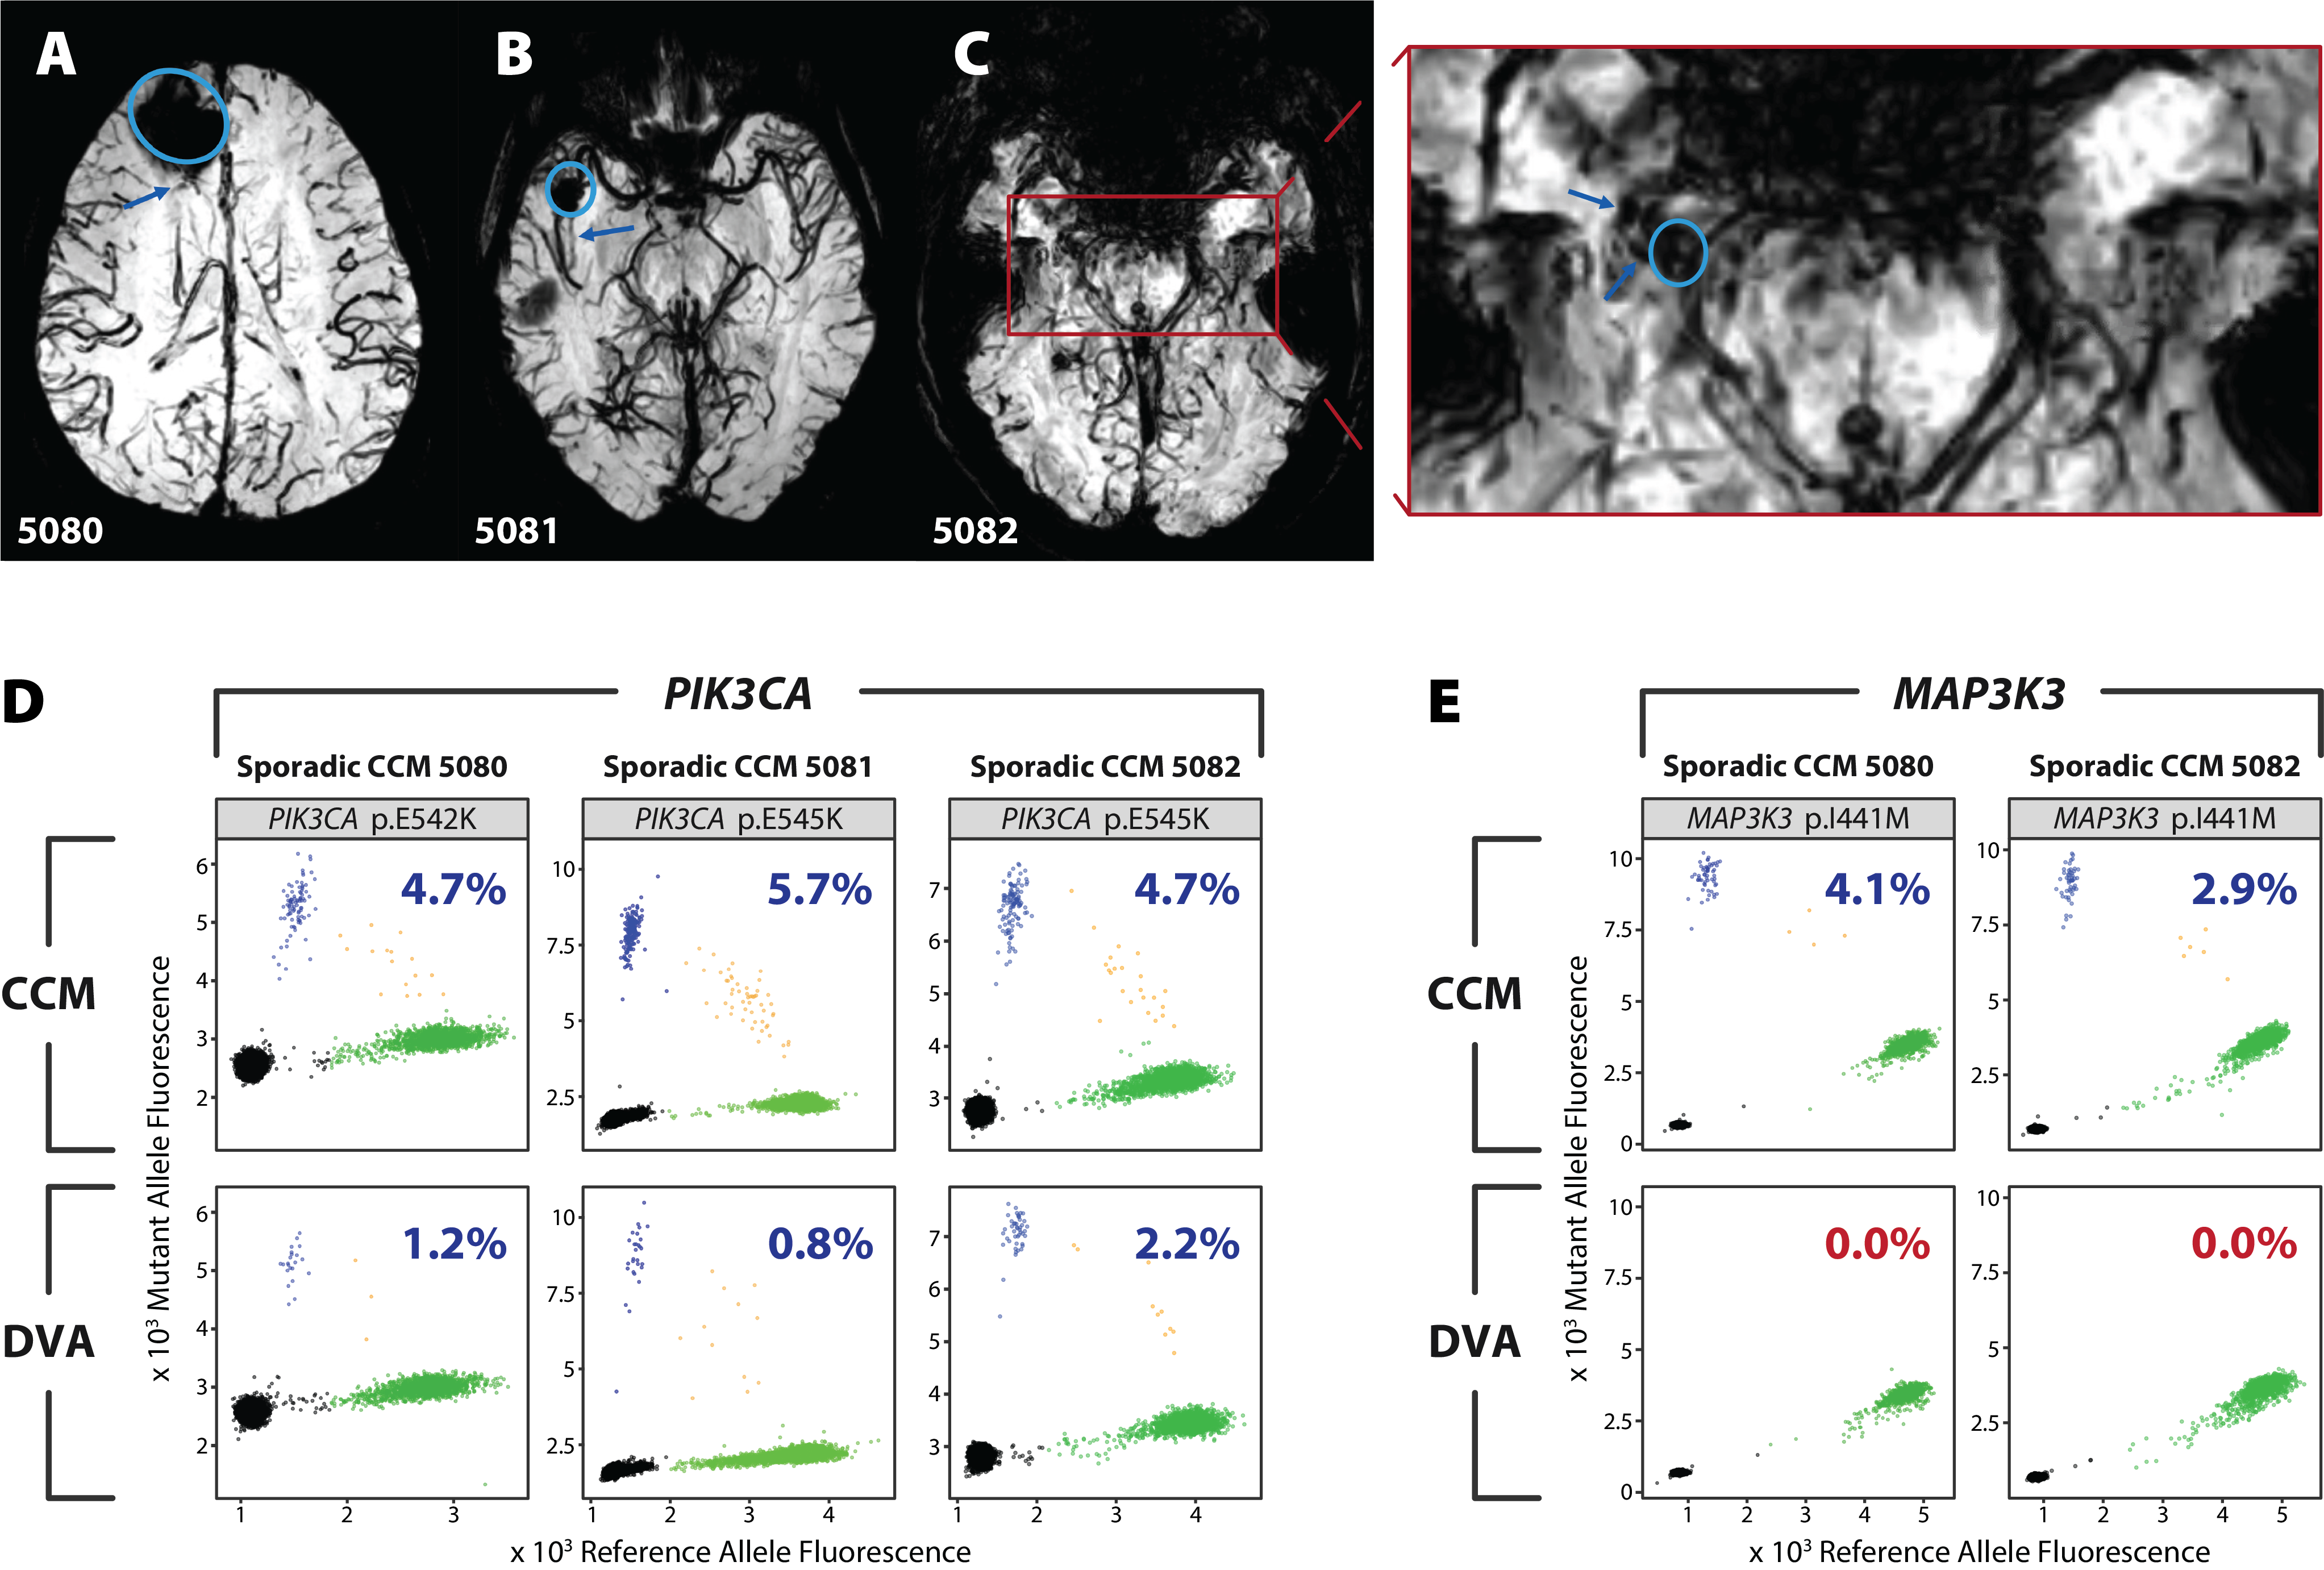
\includegraphics[width=5.8in]{MAP_DVA}
\caption[CCM and Adjacent DVA Have Identical \italicize{PIK3CA} Mutations]{\textbf{CCM and Adjacent DVA Have Identical \italicize{PIK3CA} Mutations.}
\textbf{A--C}. Axial magnetic resonance (MR) susceptibility weighted images acquired at 3 Tesla showing CCM (circle) and associated DVA branches sampled during surgery (arrow) in individuals with CCM 5080 (A) or 5081 (B) or 5082(C). The inset red box in C shows the region expanded to the right with the CCM and DVA marked. \textbf{D--E}. Somatic mutations in \italicize{PIK3CA} (D) and \italicize{MAP3K3} (E) in CCM (top panels) and the associated DVA (bottom panels) from samples 5081, 5082, and 5083. Mutations were detected by droplet digital PCR (ddPCR) and shown as the fluorescence of the reference probe on the x-axis, and the mutant probe on the y-axis. Droplets containing the reference allele, mutant allele, both, or neither, are colored in green, blue, orange, and black respectively. Percentage inset into each graph shows the variant allele frequency for the displayed mutation. If the mutation was determined to be present, the percentage is blue, else the percentage is red.}

\label{MAP_DVA}
\end{figure}
%%%%%%%%%%%%%%%%%%%%%%%%%%%%%%

\subsection{Cellular Phase of Somatic \italicize{MAP3K3} and \italicize{PIK3CA} Mutations}

While somatic mutations in \italicize{KRIT1}, \italicize{CCM2}, \italicize{PDCD10}, and \italicize{MAP3K3} are mutually exclusive, somatic gain of function mutations in \italicize{PIK3CA} may co-occur with any other mutation (Figure~\ref{MAP_discovery}A). We have previously shown that co-occurring mutations in \italicize{KRIT1}/\italicize{CCM2} and \italicize{PIK3CA} occur in the same clonal population of cells \citep{ren2021}. To determine whether \italicize{MAP3K3} and \italicize{PIK3CA} mutations co-exist in the same cells we performed single-nucleus DNA-sequencing (snDNA-seq) on frozen tissue from three surgically resected CCMs determined to harbor both mutations (Figure~\ref{MAP_discovery}B--D). 

In CCMs 5002 and 5030, the vast majority of mutant nuclei harbor both mutations in \italicize{MAP3K3} and in \italicize{PIK3CA} indicating that these mutations co-exist in the same cells. In CCM 5032, 37\% (19/51) of mutant nuclei harbor both mutations. While this is a far lower fraction compared to other samples, it is significantly higher than may be expected by chance when sampling from 1405 total nuclei (\italicize{P} = $1.3\times10^{-05}$, Figure~\ref{MAP_discovery}E). In bulk genetic analysis, the allele frequencies of \italicize{PIK3CA} and \italicize{MAP3K3} mutations detected in CCM 5002 were 19\% and 13\% respectively. In snDNA-seq the allele frequencies of these mutations increased to 54\% and 55\% respectively. This difference likely reflects the mosaic nature of CCMs. As snDNA-seq requires nuclei harvested from frozen tissue, we must sample a new area of the frozen lesion than was sampled for bulk sequencing. Sampling from different sites of the same lesion often results in minor changes in allele frequency, however the drastic change in allele frequency we find in CCM 5002 suggests either that our initial sample of the lesion for bulk sequencing contained largely non-lesion tissue, or an uneven distribution of mutant cells in the lesion. 

\subsection{CCMs and DVA Harbor a Shared Mutation in \italicize{PIK3CA} }

Many sporadic CCMs are found in the vicinity of a developmental venous anomaly (DVA). We hypothesized that CCM and DVA may have a common genetic origin, specifically that DVA may be a genetic precursor to CCM. To determine whether DVA and CCMs originate from a shared mutation, we collected three sporadic CCMs and sampled a portion of the associated DVA obtained during surgery (Figure~\ref{MAP_DVA}A--C). Assays for mutations via ddPCR revealed that all three CCMs have a somatic activating mutation in \italicize{PIK3CA} and that the same mutation is present within the paired DVA samples at lower frequency (Figure~\ref{MAP_DVA}D). Furthermore, ddPCR revealed that two of the CCMs harbored a mutation in \italicize{MAP3K3} in addition to the previously noted mutation in \italicize{PIK3CA}. However, unlike the \italicize{PIK3CA} mutation, the \italicize{MAP3K3} mutation was entirely absent from both DVA samples (Figure~\ref{MAP_DVA}E). The presence of the \italicize{PIK3CA}, but not the \italicize{MAP3K3}, mutation in the DVA confirms that the \italicize{PIK3CA} mutation in the DVA did not arise via cross-sample contamination. The presence of multiple somatic mutations in these CCMs allows us to infer the developmental history of the lesion. The cancer field commonly uses the presence or absence of somatic mutations in clonal populations to track the evolutionary history of a tumor \citep{jiao2014, loo2018}. Recent studies have expanded on this approach to use somatic mutations as endogenous barcodes to track embryonic development \citep{bizzotto2021}. Using this same approach, we infer that the DVA was the first lesion to develop and that the associated CCM is derived from cells of the DVA following a somatic mutation in \italicize{MAP3K3}. 

\subsection{Plasma miRNAs Reflect PI3K Activation in DVA Patients}

In addition to assaying the presence of \italicize{PIK3CA} mutations in DVA associated with CCM, we would ideally also assay DVA that are not associated with CCM. Unfortunately, DVA are benign malformations and are not resected unless associated with an additional pathology. This has precluded the direct assessment of \italicize{PIK3CA} mutations in DVA without a CCM.   To address this limitation, we sought another source of tissue that could be assayed for indirect evidence of \italicize{PIK3CA} activation.  Thus, we collected plasma from individuals with DVA without a CCM and measured circulating miRNAs that might serve as biomarkers reflecting \italicize{PIK3CA} activity \citep{mori2019}.

We sequenced the plasma miRNomes of 12 individuals with a sporadic CCM associated with a DVA (CCM + DVA), 6 individuals with a DVA without a CCM (DVA only), and 7 healthy controls. Three plasma miRNAs were DE in the DVA only group when compared to healthy controls (P $<$ 0.05; false discovery rate (FDR) corrected). Two of these DE miRNAs, \italicize{miR-134-5p} (FC = 0.10) and \italicize{miR-92a-3p} (FC = 3.10), putatively target \italicize{PIK3CA} and \italicize{PIK3CB} respectively, which are both components of the PI3K/AKT/mTOR pathway (Figure~\ref{MAP_miRNA}).

In addition, 18 plasma miRNAs were DE in CCM + DVA when compared to DVA only (P $<$ 0.05; FDR corrected). Two of the 18 DE miRNAs, \italicize{miR-122-5p} (FC = 5.25) and \italicize{miR-182-5p} (FC = 0.21), target \italicize{AKT3} and \italicize{MAP3K3} respectively, linking them to both the PI3K/AKT/mTOR and MAPK/ERK pathways. Additionally, \italicize{let-7c-5p} (FC = 12.64) targets both \italicize{PIK3CA} and \italicize{MAP3K3}, consistent with the role of these two pathways in sporadic CCM pathogenesis (Figure~\ref{MAP_miRNA}). Of interest, \italicize{let-7c-5p} also targets \italicize{COL1A1}, a DEG within the transcriptome of human sporadic CCM lesions (see Supplementary Data). This gene is associated with PI3K/AKT signaling, platelet activation, and ECM-receptor interaction KEGG pathways \citep{kanehisa2021, kanehisa2000}, all of which have previously been implicated in CCM disease \citep{faurobert2013, hong2021, ramirez2019, ren2021}.

Additionally, 28 DE plasma miRNAs were identified between CCM + DVA and healthy controls (P $<$ 0.05; FDR corrected). Four of these miRNAs putatively target \italicize{PIK3CA}: \italicize{miR-148a-3p} (FC = 3.27), \italicize{miR-148b-3p} (FC = 2.64), \italicize{miR-128-3p} (FC = 2.55) and \italicize{let-7c-5p} (FC = 4.20), which also targets \italicize{MAP3K3}. 

%%%%%%%%%%%%%%%%%%%%%%%%%%%%%%
%				     FIGURE 3					%
%%%%%%%%%%%%%%%%%%%%%%%%%%%%%%
\begin{figure}[t!]
\centering
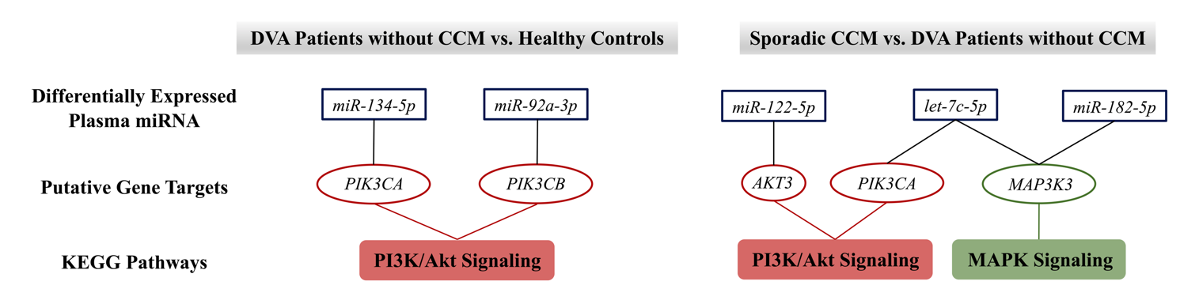
\includegraphics[width=6in]{MAP_miRNA}
\caption[Differentially Expressed micro-RNAs in CCM and DVA]{\textbf{Differentially Expressed micro-RNAs in CCM and DVA. \\} 
Two miRNAs differentially expressed (DE) in the plasma of individuals with DVA without a CCM, \italicize{miR-134-5p} and \italicize{miR-92a-3p}, putatively target genes in the Kyoto Encyclopedia of Genes and Genomes (KEGG) PI3K/AKT signaling pathway. In the plasma of individuals with sporadic CCMs with an associated DVA, \italicize{miR-122-5p}, \italicize{miR-182-5p}, and \italicize{let-7c-5p} were DE and found to target genes within both PI3K/AKT and MAPK signaling KEGG pathways. All results were P $<$ 0.05; false discovery rate corrected. }

\label{MAP_miRNA}
\end{figure}
%%%%%%%%%%%%%%%%%%%%%%%%%%%%%%


\subsection{Relative Probability of Multiple Somatic Mutations }

The association between DVA and sporadic---but not familial---CCMs suggests that there are at least two genetic trajectories by which a CCM may develop. The first trajectory is via a quiescent CCM caused by an initial mutation in \italicize{KRIT1}, \italicize{CCM2}, \italicize{PDCD10}, or \italicize{MAP3K3}. The second trajectory is via a DVA caused by an initial mutation in \italicize{PIK3CA} with subsequent mutations in \italicize{KRIT1}, \italicize{CCM2}, \italicize{PDCD10}, or \italicize{MAP3K3} leading to CCM formation. To understand whether one trajectory is favored in familial vs sporadic CCMs we use a simplified model to estimate the relative probability of CCM complex LOF (\italicize{KRIT1}, \italicize{CCM2}, \italicize{PDCD10}), \italicize{MAP3K3} GOF, and \italicize{PIK3CA} GOF. 

%%%%%%%%%%%%%%%%%%%%%%%%%%%%%%
%				     FIGURE 4					%
%%%%%%%%%%%%%%%%%%%%%%%%%%%%%%
\begin{figure}[t!]
\centering
\includegraphics[scale=.19]{MAP_model}
\caption[Genetic Model of CCM Pathogenesis]{\textbf{Genetic Model of CCM Pathogenesis. \\} 
The genetic trajectories that underly familial and sporadic CCM pathogenesis. The initial path of familial and sporadic CCMs are denoted by arrow colors (green and orange respectively) with the relative probability of each path denoted by the size of the arrow. Familial CCM preferentially develop via a LOF mutation in the CCM complex (\italicize{KRIT1}, \italicize{CCM2}, \italicize{PDCD10}) to develop a quiescent CCM that may acquire an additional mutation in \italicize{PIK3CA} that drives lesion growth. Sporadic CCM are more likely to develop via a DVA caused by a \italicize{PIK3CA} mutation creating a clonal population of cells that may subsequently acquire a CCM complex LOF or \italicize{MAP3K3} GOF. }

\label{MAP_model}
\end{figure}
%%%%%%%%%%%%%%%%%%%%%%%%%%%%%%

Somatic mutagenesis is a complex process that depends on many variables including cell turnover rates, age, exposure to mutagens, and numerous genetic factors which facilitate DNA synthesis and repair. As a result, estimating absolute mutation rate is not feasible. However, by assuming a uniform mutation rate across these genes, we can determine the relative rate of CCM complex LOF, \italicize{MAP3K3} GOF, and \italicize{PIK3CA} GOF as simply the number of mutations that result in LOF or GOF. Determining this value for \italicize{MAP3K3} and \italicize{PIK3CA} is straightforward. To date there is only a single mutation in \italicize{MAP3K3} (p.I441M) that has been reported in CCMs. The spectrum of mutations in \italicize{PIK3CA} has been well documented in the catalogue of somatic mutations in cancer (COSMIC). In the absence of functional assays for each mutation, we define a GOF mutation as any mutation that accounts for $>$1\% of all \italicize{PIK3CA} mutations COSMIC which was determined to be 10 mutations. The number of CCM complex LOF mutations was determined by considering all possible single nucleotide variants that would result in a premature stop codon or disrupt a canonical splice site (see Methods). The average of these values for all three genes is 430 mutations (\italicize{KRIT1} = 718, \italicize{CCM2} = 353, \italicize{PDCD10} = 220). This is a very conservative estimate and should be considered a lower bound, since the majority of CCM complex LOF mutations are the result of frameshift mutations which are not accounted for here. 

From the relative probability of each mutation, it is clear that familial CCMs will almost always develop via CCM complex LOF (Figure~\ref{MAP_model} top), consistent with the lack of association between familial CCM and DVA. The probability of two CCM complex LOF mutations in trans and in the same cell (as required for CCM complex LOF in sporadic CCMs) is far lower than for a single mutation (as required for CCM complex LOF in familial CCMs). In this study we identified 6 sporadic CCMs with biallelic somatic mutations in a CCM complex gene, therefore probability of this event is likely of similar magnitude to \italicize{MAP3K3} GOF which we identified in 15 sporadic CCMs. Assuming the same relative probability for CCM complex LOF as \italicize{MAP3K3} GOF in sporadic CCMs, we determine that sporadic CCM are at least 5x more likely to develop via \italicize{PIK3CA} GOF than CCM complex LOF or \italicize{MAP3K3} GOF (Figure~\ref{MAP_model} bottom). This finding is consistent with the strong association between DVA and sporadic CCM.



\section{Discussion}

\subsection{\italicize{MAP3K3} GOF and CCM LOF Have Similar Molecular Effects}
In this study we have further interrogated the relationship between somatic mutations in \italicize{KRIT1}, \italicize{CCM2}, \italicize{PDCD10}, \italicize{MAP3K3}, and \italicize{PIK3CA} which contribute to the pathogenesis of CCM. We find that somatic mutations in \italicize{MAP3K3} are not present in CCMs from individuals with familial CCM, consistent with a recent study \citep{weng2021}.  We find that sporadic CCMs may harbor mutations in \italicize{MAP3K3}, \italicize{KRIT1}, \italicize{CCM2}, or \italicize{PDCD10}, but that the lesion will only have mutations in one of these genes. This implies that mutations in any of \italicize{MAP3K3}, \italicize{KRIT1}, \italicize{CCM2}, or \italicize{PDCD10} are sufficient for CCM formation, without the need for mutations in a second gene. As \italicize{KRIT1}, \italicize{CCM2}, and \italicize{PDCD10} are all members of the CCM signaling complex, this reflects the fact that the loss of any component of the complex prevents normal signal transduction. Similarly, as the CCM complex is a direct inhibitor of \italicize{MAP3K3} activity \citep{zhou2015}, this pathway may be activated by either CCM complex LOF or by \italicize{MAP3K3} GOF, but the mutual exclusivity of mutations in these genes suggests that only one of these events is necessary for lesion formation. 

\subsection{DVA Clonal Expansion Promotes Additional Mutations}
CCMs often develop as the result of multiple somatic mutations that co-exist within the same cells as we show with snDNA-seq. Although several somatic mutations occur in every cell division \citep{rodin2021}, the specificity of the mutations in CCM translates to a very low chance of acquiring these mutations within a single cell. This is especially true of somatic mutations in \italicize{MAP3K3} and \italicize{PIK3CA}, both of which have very narrow spectra of activating mutations. Despite this improbability, the accumulation of these mutations in CCM seems to occur frequently. One possible explanation for this phenomenon is that CCMs have an increased rate of somatic mutations. There is little evidence supporting this theory and such a mechanism is difficult to conceive in cases of sporadic CCM where individuals have no known genetic predisposition to CCM. An alternative explanation is that after an initial somatic mutation, the singly-mutated cell undergoes clonal expansion to form an intermediate lesion. In this study we identify 7 CCMs with either biallelic LOF in a CCM complex gene or \italicize{MAP3K3} GOF in the absence a \italicize{PIK3CA} mutation, suggesting that \italicize{PIK3CA} activation is not required for CCM formation. Furthermore, previous work in mouse models has shown that loss of a CCM complex gene (with WT \italicize{Pik3ca}) leads to clonal expansion of the mutant cells and in later stages of growth, incorporation of WT endothelial cells \citep{detter2018, malinverno2019}. As a result of this clonal expansion, the probability of creating a double-mutant cell increases by a factor of the clonal population size as there are more cells in which the second mutation may occur (Figure~\ref{ClonalExpansionDiagram}). 
%%%%%%%%%%%%%%%%%%%%%%%%%%%%%%
%				     FIGURE 5					%
%%%%%%%%%%%%%%%%%%%%%%%%%%%%%%
\begin{figure}[b!]
\centering
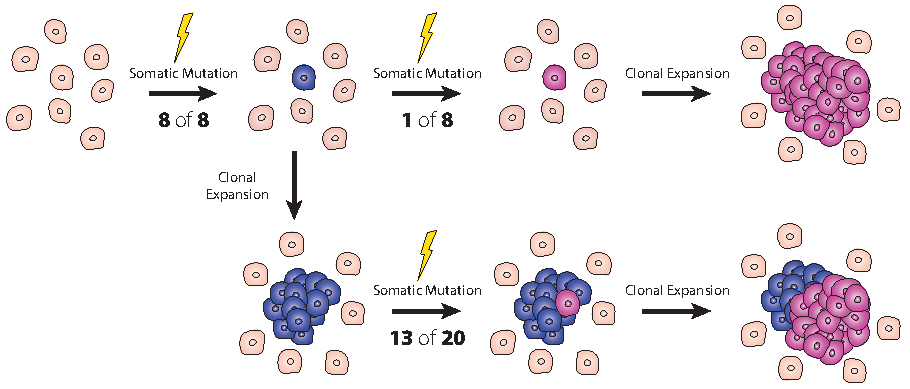
\includegraphics[width=6in]{ClonalExpansionDiagram}
\caption[Clonal Expansion Predisposes to Additional Mutations]{\textbf{Clonal Expansion Predisposes to Additional Mutations. \\} A schematic showing the probability of acquiring two somatic mutations with or without an intermediate clonal expansion step. In this example a single cell with an initial somatic mutation either remains quiescent (top) or clonally expands (bottom). The probability that a subsequent mutation occurs in a cell with the initial mutation increases by a factor of the mutant population (1 cell in top, 13 cells in bottom).}

\label{ClonalExpansionDiagram}
\end{figure}
%%%%%%%%%%%%%%%%%%%%%%%%%%%%%%
Somatic mutations in this clonal population may be acquired by genome replication during expansion or after expansion as mutations accumulate via DNA damage and error-prone repair as has been reported in other quiescent cell types \citep{lodato2018}. 

The data presented in this study suggest that DVA are an intermediate lesion as posited by the latter explanation. Genetic analysis of DVA and paired CCM show that at least some DVA develop following a somatic activating mutation in \italicize{PIK3CA}. Furthermore, plasma miRNA analysis of individuals with DVA-associated CCM revealed differentially expressed miRNAs that putatively target \italicize{PIK3CA} and \italicize{MAP3K3}, the same genes that are mutated in these lesions. By contrast, individuals with DVA but no CCM differentially expressed miRNAs that putatively target \italicize{PIK3CA}, but not \italicize{MAP3K3}. These data are consistent with the distribution of mutations we observe in CCM and DVA, and the differential regulation of these miRNAs may reflect an attempt to compensate for dysregulation of PI3K and MAPK signaling due to the somatic mutations. 

The presence of \italicize{PIK3CA} mutations in DVA suggests that DVA act as a genetic precursor to CCM, which would account for the strong association between sporadic CCM and DVA. Likewise, DVA are not associated with familial CCM because the presence of an inherited germline mutation in a CCM gene strongly biases probability towards a CCM gene somatic mutation occurring first, as there exist many different mutations that may cause LOF, but far fewer that would cause GOF in \italicize{PIK3CA}. 

This study is the first to collect CCM and associated DVA for genetic analysis. Collecting tissue from CCM-associated DVA is challenging; however, collecting tissue from DVA not associated with CCM is yet more challenging as DVA are considered benign and are therefore not resected. We have attempted to address this limitation by studying biomarkers of PI3K activity which can be assayed noninvasively in blood plasma. Assaying the presence of \italicize{PIK3CA} mutations in DVA not associated with CCM will be the domain of future studies, but the data we present here demonstrate a clear link between DVA and \italicize{PIK3CA}, and suggest a model that explains the long recognized\textemdash but poorly understood\textemdash association between CCM and DVA. 

\subsection{DVA May Contribute to Additional Phenotypes}
While we are unable to address the presence of \italicize{PIK3CA} mutations in DVA not associated with CCM, it is worth noting that DVAs have been associated with other PI3K-related disorders\citep{brinjikji2018, dhamija2018, rasalkar2010, roux2020, santucci2008, tan2007, ucler2019} including some cancers and neurological malformations, suggesting that DVA may have a role, possibly even as a genetic primer, in these other diseases. 



\section{Methods}
\subsubsection{Sample Collection}
	Surgically resected CCMs were obtained from the University of Chicago, the Barrow Neurological Institute, and the Angioma Alliance biobank. Additional DVA tissue was discretely dissected from the lesion during surgical resection of the associated CCM at the University of Chicago. This study was approved by each institution’s respective Institutional Review Board. 

\subsubsection{DNA Extraction}
	DNA from CCM and DVA samples was extracted using the DNeasy blood and tissue kit (QIAGEN, catalog number 69504) per the manufacturers protocol. DNA purity was determined by Nanodrop and concentration was determined using the Qubit dsDNA BR assay kit (Invitrogen, catalog number Q32850) per the manufacturers protocol. 

\subsubsection{Droplet Digital PCR}
Detection of \italicize{MAP3K3} p.I441M was performed via ddPCR using a previously described probe set\citep{couto2015}. Assays were performed using 30--100ng of DNA with the QX200 AutoDG system (BioRad) and quantified with the QX200 droplet reader (BioRad). Analysis was performed with the QuantaSoft software (BioRad). 

\subsubsection{Sequencing}
	A total of 8 sporadic CCMs with no identified mutation in \italicize{KRIT1}, \italicize{CCM2}, \italicize{PDCD10}, or \italicize{MAP3K3} (5001, 5005, 5006, 5022, 5024, 5036, 5078, and 5081) were used for whole-exome sequencing prepared using the SureSelect Human All Exon V7 probe set (Agilent, Design ID S31285117) per the manufacturers protocol. Prepared libraries were sequenced on one lane of a NovaSeq 6000 S4 flow cell for a mean depth of 133x. 

\subsubsection{Sequence Analysis}
	Sequencing data was processed using the Gene Analysis Toolkit (GATK, Broad Institute) while following the GATK best practices for somatic short variant discovery using Mutect2. Secondary variant detection was performed using gonomics (https://github.com/vertgenlab/gonomics) and bcftools mpileup to manually examine \italicize{KRIT1}, \italicize{CCM2}, \italicize{PDCD10}, and \italicize{MAP3K3} for somatic variants. Putative variants were annotated using Funcotator (GATK), the catalog of somatic mutation in cancer (COSMIC), and the genome aggregation database (gnomAD). Putative variants were filtered according to the following criteria: greater than 50x total coverage, less than 90\% strand specificity, greater than 5 reads supporting the alternate allele, greater than 1\% alternate allele frequency, less than 1\% population allele frequency, and predicted protein/splicing change. 

\subsubsection{Single-Nucleus DNA Sequencing}
Nuclei isolation, snDNA-seq, and analysis were performed as previously described\citep{ren2021}. 

\subsubsection{miRNA Extraction and Sequencing}
Total plasma RNA was extracted from the plasma of 12 individuals with a sporadic CCM and an associated DVA (CCM + DVA), 6 individuals with DVA and without a CCM (DVA only), and 7 healthy controls using the miRNeasy Serum/Plasma Kit (Qiagen, Hilden, Germany) following the manufacturer isolation protocol. Diagnosis of CCM with an associated DVA, as well as DVA without a CCM lesion was confirmed on susceptibility weighted MR imaging. Illumina small RNA-Seq kits (Clontech, Mountain View, CA, USA) were then used to generate cDNA libraries, and sequencing was completed with the Illumina HiSeq 4000 platform (Illumina, San Diego, CA, USA), with single-end 50bp reads, at the University of Chicago Genomics Core. Differential miRNA analyses were completed between (1) CCM + DVA to DVA only and then (2) DVA only to healthy controls. The differentially expressed miRNAs were identified having P $<$ 0.05, FDR-corrected. All analyses were completed using the sRNAToolbox and DESeq2 R packages\citep{love2014, rueda2015}.

\subsubsection{Identification of Putative Targets}
miRWalk 3.0 was used to identify the putative gene targets of each of the DE miRNAs, using a random forest tree algorithm with a bonding prediction probability higher than 95\% on the 3 different gene locations (3' UTR, 5' UTR, and CDS)\citep{sticht2018}. Putative gene targets of the DE miRNAs were identified in at least 2 of the 3 databases. DE miRNAs between (1) CCM + DVA and DVA only as well as (2) DVA only and healthy controls were then analyzed for potential targeting of the PI3K, AKT, and MAPK gene families. 

\subsubsection{Estimating Possible LOF Mutations in \italicize{KRIT1}, \italicize{CCM2}, and \italicize{PDCD10}}
The majority of LOF mutations in \italicize{KRIT1}, \italicize{CCM2}, and \italicize{PDCD10} result in either: creation of a premature stop codon (nonsense); disruption of a canonical splice site; or a frameshift. The first two of these are typically caused by a single nucleotide variant (SNV) and can be determined from the gene sequence. However, frameshift variants resulting from insertions and deletions may occur in any exon regardless of sequence context. This prevents a meaningful comparison between indel and SNV events, without making assumptions about the rate of somatic SNV and indel events. To determine a conservative lower bound for the number of LOF mutations in the CCM complex genes, we only consider nonsense and splice site mutations. The number of nonsense and splice site mutations were determined from the sequences of \italicize{KRIT1} (ENST00000394507.5), \italicize{CCM2} (ENST00000258781.11), and \italicize{PDCD10} (ENST00000392750.7). Nonsense mutations were considered any SNV in the coding sequence that would result in an in frame stop codon prior to the stop codon in the reference sequence. Splice site mutations were considered any SNV in the nearly invariant sequences at each exon-intron boundary that mediate canonical splicing. 
	
\subsubsection{Sporadic CCM Transcriptome}
Laser micro-dissected neurovascular units (NVUs) from sporadic CCM lesions were sequenced for transcriptomic analyses in comparison to micro-dissected NVUs from human brain microvasculature. The differential analyses identified 426 DE genes (DEGs) (P $<$ 0.05; FDR corrected; FC $>$ $\vert$1.5$\vert$). Additionally, 8 pathways from the Kyoto Encyclopedia of Genes and Genomes (KEGG) were enriched (P $<$ 0.05, FDR corrected).  


\subsubsection{Sporadic Transcriptome and KEGG Pathway Analyses}

Six human sporadic CCM lesions were surgically resected prior to embedding in optimal cutting temperature, snap-freezing, and storing at -80$^{\circ}$C. Control brain tissue was collected during autopsy from three subjects lacking neurological disease, fixed in formalin, and embedded in paraffin blocks. Five-\textmu m tissue sections were mounted on Leica glass slides (Leica Biosystems Inc) and were stained, in accordance with the manufacturer’s protocols, with HistoGene (Applied Biosystems) for frozen tissue and Paradise stain (Applied Biosystems) for paraffin-embedded tissue. The neurovascular units (NVUs) from sporadic CCM lesions and normal brain capillaries were then collected using laser capture microdissection and stored at -80$^{\circ}$C. RNA was isolated using an RNA extraction kit (RNeasy Micro Kit, Qiagen). cDNA libraries were then generated with low-input strand-specific RNA-Seq kits (Clontech) and sequenced using the Illumina HiSeq 4000 platform with single-end 50bp reads. Differentially expressed genes were defined as P $<$ 0.05, FDR corrected. 

Enriched Kyoto Encyclopedia of Genes and Genomes (KEGG) pathways\citep{kanehisa2021, kanehisa2000} were obtained for the DE genes (DEGs) in the sporadic transcriptome with fold change values greater than 1.5 (P $<$ 0.05, FDR corrected). The sporadic transcriptome was compared to the putative targets of the DE miRNAs between (1) CCM + DVA and DVA only as well as (2) DVA only and healthy controls to obtain a set of overlapping genes. Enriched Kyoto Encyclopedia of Genes and Genomes (KEGG) pathways were obtained for the overlapping genes, using a database and knowledge extraction engine with a Bayes factor greater than 3. 

\section{Contributions and Acknowledgements}
This chapter is adapted from a study published in \italicize{bioR$\chi$iv} (Snellings et al., 2021) with the following authors: Daniel A. Snellings, Romuald Girard, Rhonda Lightle, Abhinav Srinath, Sharbel Romanos, Ying Li, Chang Chen, Aileen A. Ren, Mark L. Kahn, Issam A. Awad, Douglas A. Marchuk. DAS designed and performed the genetic studies of human CCM lesions and wrote the manuscript. IAA performed surgical resection of CCM and DVA samples used in this study. RG, RL, AS, SR, YL, CC and IAA performed plasma miRNA sequencing and analysis. AAR and MLK assisted with experimental design. RG, IAA, and DAM designed experiments and wrote the manuscript.

We thank the patients who donated tissue for this study. We thank Angioma Alliance, the Barrow Neurological Institute, and the University of Chicago for patient enrollment and sample collection. Nucleus sorting was performed in the Duke Human Vaccine Institute Research Flow Cytometry Shared Resource Facility. We thank Duke University School of Medicine for use of the Sequencing and Genomic Technologies Shared Resource for library preparation and sequencing. These studies were supported by National Institute of Health grants, P01NS092521 (DM, IA, MK), F31HL152738 (DS).
}
\chapter{Conclusions \& Musings}

\section{HHT Pathogenesis}

\section{CCM Pathogenesis}
\subsection{CCM \& Meningioma}
Although the vascular lesions are the primary sequelae of familial CCM, many groups have noted an increased prevalence of meningioma in individuals with familial CCM—especially those with a mutation in \italicize{PDCD10} \citep{labauge2009, riant2013, garaci2015}. 

\section{Developmental Venous Anomalies as a Primer for Disease}
\subsection{Association with Sporadic CCM}
\subsection{Association with Other Diseases}
\subsection{Cowden Syndrome}
\subsection{Implications}

\section{Other Vascular Malformations}
\subsection{Classification of Vascular Malformations and Vascular Tumors}

\subsection{Sturge-Weber Syndrome and Somatic Mutations in \italicize{GNAQ}}
\subsubsection{Happle's hypothesis}
\subsubsection{\italicize{GNAQ} in uveal melanoma and circumscribed choroidal hemangioma}
\subsubsection{Link between SWS, UM, and CCH?}

\subsection{The Curious Case of Infantile Hemangioma}
Infantile hemangioma (IH) are one of the most common vascular malformations. They occur in children and are typically present at birth as a red spot flush with the surrounding skin. Soon after birth the hemangioma rapidly grows and becomes raised from the skin. They are generally benign and are typically left alone unless they cover the child's mouth, nose, or eyes. What makes IH so interesting compared to other types of vascular malformations is that they almost always completely regress within the first few years of the child's life. While other types of vascular malformations may spontaneously regress (telangiectasia and AVMs), none do so with the consistency of IH. This phenomenon has been of great interest, not for the purpose of developing therapeutics for IH (propranolol is an extremely effective treatment for IH) but for uncovering the mechanism of regression in the hopes that what we learn can be applied to regress other, more nefarious, vascular malformations. 
\subsubsection{GLUT1 in IH endothelium}
Perhaps one of the most provocative discoveries into the mechanism of IH pathogenesis is the fact that endothelial cells from IHs highly express GLUT1 \citep{north2000, north2001}. GLUT1 is a glucose transporter that has remarkable specificity for the placental endothelium. This finding suggested that the IH may be comprised of cells that dislodged from the maternal placenta, then became hyper-proliferative in a post-fetal environment. If this hypothesis is correct, one would expect to find that the IH is a genetically chimeric growth between fetal and maternal cells. This hypothesis was put to the test using fluorescence \italicize{in situ} hybridization to assay the presence of XX cells in IH from a male infant with confirmation by sequencing microsatellites and SNPs that were divergent between mother and child. This analysis found no evidence for maternal-fetal chimerism in IH \citep{pittman2006}. Despite this counter-evidence, the presence of GLUT1 in IH is strongly indicative of some link with the placenta though unfortunately this link currently remains elusive.
\subsubsection{Efforts to find somatic mutations in IH}
As it is quickly becoming clear that the vast majority of vascular malformations are the result of somatic mutations—many occurring in known oncogenes—I thought that somatic mutations may also underlie IH. To test this, I sequenced 61 IH lesions on an 'oncopanel' covering many genes that are highly mutated in cancers as well as several genes previously implicated in vascular malformations (\italicize{KRIT1, CCM2, PDCD10, ACVRL1, ENG, SMAD4,} etc.) Unfortunately after filtering putative variants, no there were no variants with likely functional significance and that occurred in more than a single sample. I am aware of at least 1 other group that has attempted to identify somatic mutations in IH via whole-exome sequencing, however to date there are no known somatic mutations in IH. One important aspect of these studies that must be noted is that they are invariably focused on coding regions of the genome. Non-coding variants are more than capable of causing disease however discovery-focused sequencing studies often ignore non-coding regions both because of the cost of sequencing the entire genome to a depth sufficient to detect somatic mutations, and the challenges associated with functional analysis of non-coding variants. Further studies may find that somatic mutations do cause IH, but they occur in a region of the genome that is missed by the majority of sequencing studies. 

\section{The Molecular Basis of Genetic Dominance}
\subsection{Phenotypic Dominance $\neq$ Genetic Dominance}
\subsection{Knudsons Fingerprint}
\subsection{The Diverse Functional Effects of Genetic Mutations}

\section{The Intersection of Somatic Mutagenesis and Evolution}
\subsection{The Creation of New Alleles}
\subsection{The Relationship Between Mutability and Fitness Landscape}
\subsection{Recurring Mutations \& Convergent Evolution}
\subsection{Clonal Evolution of Somatic Mutants}
\subsection{Cancer}

\section{Somatic Mutations}
\subsection{The Role of Somatic Mutations in Aging}
\subsection{Constitutional Intolerance \& Somatic Permissiveness}
\subsection{Somatic Reversion of Pathogenic Mutations}
\subsection{What is the Consequence of RNA Mutations?} 
%mutations at the RNA level i.e. individual mutant RNA molecules
%interactions with the ribosome?
%could a single RNA molecule screw things up?

\section{Innovation in the Sequencing Era}
\subsection{Detection of Somatic Mutations}
\subsection{Single Cell Sequencing}
\subsection{Utility of Rare Disease Research in Mechanistic Discovery}
\subsection{Data Democratization \& Individual Privacy}
\subsection{Growing Importance of Informatics in Biology}}
%==============================================================================

%-----------------------------------------------------------------------------%
% APPENDICES -- OPTIONAL. These are just chapters enumerated by Appendix A,
%                Appendix B, Appendix C...
%-----------------------------------------------------------------------------%
\appendix
\chapter{Probability of Somatic Mutations}
\clearpage

When describing my results to colleagues I am often met with the questions: ``How can so many somatic mutations be occurring? Could these lesions have an elevated mutation rate?". Though our intuition says it cannot be possible, I maintain that the somatic mutations I find in telangiectasia are the result of random chance via normal mutagenic processes. Unfortunately, too little is known about the rates of mutagenesis across the genome and in different tissues to accurately quantify the probability of these events. Despite this limitation, in this Appendix I attempt to conservatively estimate the probability of the events I describe in Chapter 2. The goal of this exercise is solely to highlight the disconnect between intuition and reality by showing that the empirically determined rate of disease is of similar magnitude to my conservative estimations. 



\section{Two-Hit Mutations in HHT}
In this section we consider the probability of biallelic loss of function (LOF) occurring in a single cell of an individual with HHT. For this exercise we will assume the individual has a germline heterozygous mutation in \italicize{ENG}. The probability of a somatic mutation resulting in biallelic LOF in a single cell ($\italicize{ENG}_{sc}^{-/-}$) is a function of the somatic mutation rate ($\mu_{som}$), the probability a mutation falls in the CDS of \italicize{ENG} ($\italicize{ENG}_{CDS}$), results in LOF, and is in \italicize{trans} with the germline mutation ($0.5$ for diploid organisms) per somatic single-nucleotide variant (sSNV) such that
\begin{equation*}
P(\italicize{ENG}_{sc}^{-/-}) = \mu_{som} \cdot \frac{P(\italicize{ENG}_{CDS}) \cdot P(LOF) \cdot 0.5}{sSNV}
\end{equation*}

Empirical data for $\mu_{som}$ is not available for endothelial cells, however $\mu_{som}$ has been evaluated for neurons via single-cell whole-genome sequencing \citep{lodato2018} and was determined to be roughly 40 sSNV per year of life ($sSNV/year$). As mutation rates are tightly linked to DNA synthesis, the values from neurons should suffice as a conservative estimate of the $\mu_{som}$ for endothelial cells. 

Assuming that the rate of somatic mutations in \italicize{ENG} matches the genome-wide average, then 
\begin{equation*}
P(\italicize{ENG}_{CDS}) = \frac{ENG~CDS~Length}{Human~Genome~Size} = \frac{1977 bp}{3.23 \times 10^9 bp} = 6.1 \times 10^{-7}
\end{equation*}

Determining whether a given mutation may result in LOF is difficult as the effects of missense and silent variants are hard to predict. Therefore here we will only consider nonsense mutations, which will almost always result in LOF. Of the 5931 possible sSNVs in the CDS of \italicize{ENG}, 507 of them result in the creation of a premature stop codon (see \url{https://github.com/dasnellings/lofprob} for code). Therefore,
\begin{equation*}
P(LOF) = \frac{507}{5931} = 0.085
\end{equation*}

Replacing these values in the original equation yields
\begin{equation*}
P(\italicize{ENG}_{sc}^{-/-}) = \frac{40~sSNV}{year} \cdot \frac{6.1 \times 10^{-7} \cdot 0.085 \cdot 0.5}{sSNV} = \frac{1.0 \times 10^{-6}}{year}
\end{equation*}

So every year, there is a 1 in 1,000,000 chance of biallelic LOF in \italicize{ENG} per cell. While this is a very low probability, consider that there are an estimated $1 \times 10^{12}$ endothelial cells in an adult human \citep{jaffe1987}. This suggests that 1,000,000 endothelial cells in an adult with HHT acquire biallelic LOF in \italicize{ENG} every year. Although the values I used for mutation rate and probability of LOF are almost certainly underestimates, the result is still many orders of magnitude higher than what we may expect. The most aggressive cases of HHT have hundreds of telangiectasia---not millions. This discrepancy likely reflects the fact that not all endothelial cells have the capacity to form an AVM, and likely only when conditions are right. Nonetheless, this demonstrates that the mutation itself is not as unlikely as it may initially appear. 



%\section{Three-Hit Mutations in Familial CCM}
%In this section we consider the probability of biallelic loss of function in \italicize{KRIT1} \textbf{and} gain of function (GOF) in \italicize{PIK3CA} in a single cell of an individual with familial CCM (germline $\italicize{KRIT1}^{+/-}$). Using the same nomenclature as before, and adding a new term for \italicize{PIK3CA} GOF
%\begin{equation*}
%P(\italicize{KRIT1}_{sc}^{-/-};\italicize{PIK3CA}_{sc}^{GOF/+}) = \mu_{som} \cdot P(\italicize{KRIT1}_{sc}^{-/-}) \cdot P(\italicize{PIK3CA}_{sc}^{GOF/+})
%\end{equation*}

%\begin{equation*}
%P(\italicize{KRIT1}_{sc}^{-/-}) = \frac{P(\italicize{KRIT1}_{CDS}) \cdot P(LOF) \cdot 0.5}{sSNV}
%\end{equation*}

%\begin{equation*}
%P(\italicize{PIK3CA}_{sc}^{GOF/+}) = \frac{P(\italicize{PIK3CA}_{CDS}) \cdot P(GOF)}{sSNV}
%\end{equation*}

%Solving first for $P(\italicize{KRIT1}_{sc}^{-/-})$; the CDS of \italicize{KRIT1} is 2211bp and we find that there 718 possible nonsense sSNVs out of a total 6633 possible sSNVs (see \url{https://github.com/dasnellings/lofprob} for code), therefore
%\begin{equation*}
%P(\italicize{KRIT1}_{CDS}) = \frac{KRIT1~CDS~Length}{Human~Genome~Size} = \frac{2211 bp}{3.23 \times 10^9 bp} = 6.8 \times 10^{-7}
%\end{equation*}

%\begin{equation*}
%P(LOF) = \frac{718}{6633} = 0.11
%\end{equation*}

%\begin{equation*}
%P(\italicize{KRIT1}_{sc}^{-/-}) = \frac{P(\italicize{KRIT1}_{CDS}) \cdot P(LOF) \cdot 0.5}{sSNV} = \frac{6.8 \times 10^{-7} \cdot 0.11 \cdot 0.5}{sSNV} = \frac{3.7 \times 10^{-8}}{sSNV}
%\end{equation*}

%Next solving for $P(\italicize{PIK3CA}_{sc}^{GOF/+})$; the CDS of \italicize{PIK3CA} is 3204bp. As a conservative estimate of the number of sSNV that may cause GOF we will consider only the 8 that have been identified in CCM (Figure~\ref{PIK_discovery}A) of the possible 9612 sSNV.
%\begin{equation*}
%P(\italicize{PIK3CA}_{CDS}) = \frac{PIK3CA~CDS~Length}{Human~Genome~Size} = \frac{3204 bp}{3.23 \times 10^9 bp} = 6.8 \times 10^{-7} = 1.0 \times 10^{-6}
%\end{equation*}

%\begin{equation*}
%P(GOF) = \frac{8}{9612} = 8.3 \times 10^{-4}
%\end{equation*}

%\begin{equation*}
%P(\italicize{PIK3CA}_{sc}^{GOF/+}) = \frac{P(\italicize{PIK3CA}_{CDS}) \cdot P(GOF)}{sSNV} = \frac{1.0 \times 10^{-6} \cdot 8.3 \times 10^{-4}}{sSNV} = \frac{8.3 \times 10^{-10}}{sSNV}
%\end{equation*}



%\section{Three-Hit Mutations in Sporadic CCM}

%\section{Three-Hit Mutations in Sporadic CCM via DVA}










} % Start with '\chapter{Title}'
%You can always add more appendices here if you want

%-----------------------------------------------------------------------------%
% BIBLIOGRAPHY -- uncomment \nocite{*} to include items in 'mybib.bib' file
% that aren't cited in the text.  Change the style to match your
% discipline's standards.  Of course, if your bibliography file isn't called
% 'mybib.bib' you might want to change that here too :)
%-----------------------------------------------------------------------------%
%\nocite{*} - if you use this it will put EVERYTHING in your .bib file into the references even if you don't cite it in the text
\bibliographystyle{./Bibliography/apa} %Formats bibliography
\cleardoublepage
\normalbaselines %Fixes spacing of bibliography
\addcontentsline{toc}{chapter}{Bibliography} %adds Bibliography to your table of contents
\bibliography{./Bibliography/References} %your bibliography file - change the path if needed
%-----------------------------------------------------------------------------%

%-----------------------------------------------------------------------------%
% BIOGRAPHY -- Start file with '\biography'.  Mandatory for Ph.D.
%-----------------------------------------------------------------------------%
\biography

Daniel Aaron Snellings was born in La Plata, Maryland on the 23\textsuperscript{rd} of October, 1995. He graduated from the Pennsylvania State University in 2017 with a Bachelor of Science in Biochemistry and Molecular Biology. Daniel entered Duke in 2017 through the Cell and Molecular Biology graduate program and joined the lab of Douglas A. Marchuk in 2018. Daniel was awarded a Ruth L. Kirschstein predoctoral fellowship from the NHLBI in 2020. In 2021, Daniel was selected as a featured plenary speaker for the annual meeting of the American Society of Human Genetics and there was selected as a semifinalist for the Charles J. Epstein award. Daniel received a Ph.D. in Molecular Genetics and Microbiology from Duke University in 2022. In April 2022, Daniel began a postdoctoral fellowship in the lab of Christopher A. Walsh at Boston Children's Hospital.
\\\\
{\Large \textbf{Publications}} \\
\textbf{D. A. Snellings}, et al. (2022) \italicize{Nat. Cardiovasc. Res.}, in press\\
\textbf{D. A. Snellings}, et al. (2021) \italicize{Circ Res}\\ \nocite{snellings2021}
A. A. Ren \& \textbf{D. A. Snellings}, et al. (2021) \italicize{Nature}\\ \nocite{ren2021}
\textbf{D. A. Snellings}, et al. (2019) \italicize{Am J Hum Genet}\\ \nocite{snellings2019}
J. Koskimaki, et al. (2019) \italicize{Acta Neuropathol Commun}\\ \nocite{koskimaki2019}
M. R. Detter, \textbf{D. A. Snellings}, D. A. Marchuk. (2018) \italicize{Circ Res}\\ \nocite{detter2018}
C. Wang, et al. (2018) \italicize{PLoS One} \nocite{wang2018}}
%-----------------------------------------------------------------------------

% You're done :)
\end{document}
